%!TEX root = surface_reconstruction.tex
% Добавьте ссылку на файлы с текстом работы
% Можно использовать команды:
%   \input или \include
% Пример:
%    \input{mainfiles/1-section} или \include{mainfiles/2-section}
% Команда \input позволяет включить текст файла без дополнительной обработки
% Команда \include при включении файла добавляет до него и после него команду
% перехода на новую страницу. Кроме того, она позволяет компилировать каждый файл
% в отдельности, что ускоряет сборку проекта.
% ВАЖНО: команда \include не поддерживает включение файлов, в которых уже содержится команда \include,
% т.е. не возможен рекурсивный вызов \include
\newcommand*{\Source}{
    %!TEX root = ../surface_reconstruction.tex
\phantomsection
\section*{Введение} 
\addcontentsline{toc}{section}{Введение}
Проблема определения поверхности по набору точек активно изучается многие годы. Несмотря на распространение методов реконструкции поверхности, многие аспекты проблемы остаются открытыми. Одними из основных трудностей в процессе реконструкции являются сложность формы и шум.  Проекционный оператор MLS [Levin 2003] зарекомендовал себя как мощный метод реконструкции поверхности. 
Метод MLS позволяет достичь простого и эффективного представления.




%Криптосистема Мак-Элиса "--- одна из старейших криптосистем с открытым ключом. Она была предложена в 1978
%Р.~Дж.~Мак-Элисом~\cite{MCEliece}. Данная криптосистема
%основывается на $\mathbf{\mathbb {NP}}$-трудной проблеме в теории
%кодирования. Основная идея её построения  состоит в маскировке
%некоторого кода, имеющего эффективные алгоритмы декодирования, под
%код, не обладающий видимой алгебраической и комбинаторной
%структурой, такие коды принято называть кодами общего положения.
%Эта криптосистема обладает одним важным преимуществом "--- высокой
%скоростью зашифрования и расшифрования. Однако, у неё имеется
%серьёзный недостаток "--- относительно низкая скорость передачи
%($R$). Обычно у кодовых криптосистем $R<1$, тогда как у
%криптосистемы RSA скорость в точности равна $1$.
%
%В этой работе рассматривается обобщение криптосистемы
%Мак-Элиса, предложенное в 1994 коду В.М.
%Сидельниковым~\cite{Sidelnikov1}. В этой работе модификация,
%предложенная В.~М.~Сидельниковым, называется криптосистемой\\
%Мак-Элиса--Сидельникова. Криптосистема Мак-Элиса--Сидельникова
%строится на основе $u$-кратного использования кодов Рида--Маллера
%$RM(r,m)$. Она имеет высокую криптографическую стойкость, скорость
%передачи близкую к $1$ и сравнительно невысокую сложность
%шифрования секретных сообщений и расшифрования криптограмм этих
%сообщений.
%
%В работе исследуются вопросы, связанные с пространством
%эквивалентных секретных ключей, то есть секретных ключей,
%порождающих одинаковые открытые ключи, новой криптосистемы. Опишем
%краткое содержание разделов работы.
%
%В \S~1 даётся определение криптосистемы Мак-Элиса, описываются её
%секретный и открытый ключи. Приводятся алгоритмы зашифрования и
%расшифрования.
%
%В \S~2 изучается ключевое пространство криптосистемы Мак-Элиса.
%Устанавливается связь классов эквивалентностей секретных ключей с
%группой автоморфизмов линейного кода, лежащего в основе этой
%криптосистемы.
%
%В \S~3 описывается криптосистема Мак-Элиса--Сидельникова:
%секретный и открытый ключи, алгоритмы зашифрования и
%расшифрования.
%
%\S~4 посвящён ключевому пространству новой криптосистемы. В нём
%вводятся множества, необходимые для описания классов
%эквивалентности секретных ключей. Получаются нижние и верхние
%оценки на мощности  введённых множеств и на число открытых ключей
%криптосистемы Мак-Элиса--Сидельникова.
%
%В \S~5 изучается криптосистема Мак-Элиса--Сидельникова в случае
%двух блоков ($u=2$).
%
%В настоящей работе получаются нижние оценки на мощность множества
%открытых ключей криптосистемы
%Мак-Элиса--Сидельникова(теорема~\ref{t3}) при использовании
%произвольного числа блоков $u$. Для кодов Рида--Маллера с
%$u$-кратным повторением строится множество, которое, в некотором
%смысле, является аналогом группы автоморфизмов обычного кода
%Рида--Маллера, и устанавливается связь этого множества с классами
%эквивалентности секретных ключей.
%
%Для случая двух блоков ($u=2$) полностью описывается указанное
%множество при использовании кодов Рида--Маллера $RM(r,m)$
%$(r\leqslant 2,r<m)$ и матриц определённого вида
%(теоремы~\ref{theorem1},~\ref{theorem2}). Тем самым при $u=2,
%r\geqslant 2, r<m$ описываются все классы эквивалентности
%секретных ключей с представителями особого вида и вычисляются их
%мощности. Для некоторых классов эквивалентности секретных ключей
%приводятся нижние оценки на их мощность(теоремы~\ref{theorem1}
%и~\ref{theorem2}).

    \section{Обзор литературы и постановка задачи исследования}
\subsection{Реконструкция поверхности основанная на триангуляции Делоне}
В современной компьютерной графике векторно-полигональная модель является наиболее распространенной. Она применяется в системах автоматизированного проектирования, средах разработки компьютерных игр, геоинформационная системах, САПР и т. д.

Методы реконструкции поверхности основанные на триангуляции Делоне являются наиболее широко известными среди полигональных методов. Главной отличительной чертой является задание полигональной сетки треугольниками образующих граф, который обладает следующими условиями: ребра графа не пересекаются и граф обладает максимальным количеством ребер с учетом этого условия, описанная окружность для любой грани графа не содержит вершин за исключением вершин принадлежащий грани ~\cite{Скворцов}. 

\begin{figure}[h]
    \centering
    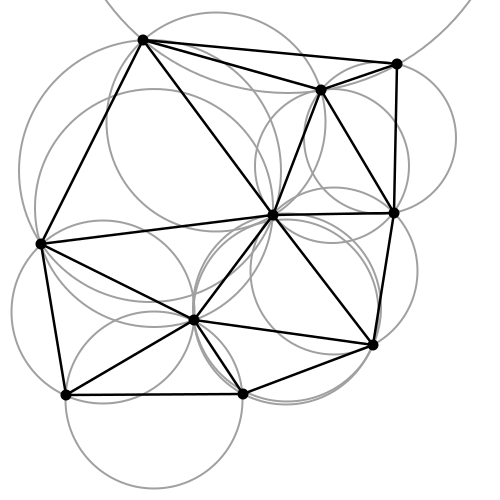
\includegraphics[scale=0.7]{images/delaunay.png}
    \caption{Выполнение инварианта триангуляции Делоне}
    \label{fig:delauney}
\end{figure}

Стоит отметить, что сами алгоритмы триангуляции не изменяют положение точек из входного облака точек. Это является слабой стороной алгоритма с точки зрения реконструкции поверхности по зашумленным входным данным. Также стоит отметить информационную зависимость алгоритмов на каждой последующей итерации от вычислений полученных на предыдущей операции, связанной с сохранением инварианта выполнения условия того, что граф является триангуляцией Делоне. Разбиение входного облака точек на сегменты ведет к последующим сложностям в соединение сегментов графа с выполнением всего того же инварианта ~\cite{Tamal}.
\subsection{Оператор локально-оптимальной проекции(LOP)}
Данный метод основан на алгоритме Вайсфельда для решения задачи Ферма-Вебера о расположении точек, также известный как многомерная медиана L1. Это статистический инструмент, который традиционно применяется во всем мире для многомерных непараметрических точечных выборок, чтобы получить хорошего представителя для большого количества выборок при наличии шума и выбросов. Эта задача была впервые сформулирована Вебером в работе ~\cite{WEBER}  под названием проблема определения оптимального местоположения. Задача состояла в том, чтобы найти оптимальное место для промплощадки, минимизирующее стоимость доступа. В статистике проблема известна как медиана L1 ~\cite{BROWN, SMALL}.

Задача Ферма-Вебера (глобальная) о расположении точек рассматривается как пространственная медиана, поскольку, будучи ограничена одномерным случаем, она совпадает с одномерной медианой и наследует некоторые ее свойства в многомерной постановке.

Реконструкция с помощью оператора проекции имеет важное достоинство: она определяет непротиворечивую геометрию на основе точек данных и предоставляет конструктивные средства для повышения ее дискретизации. 
Оператор локально-оптимальной проекции без параметризации использует более примитивный механизм проецирования, но поскольку он не основан на локальной 2D-параметризации, он более надежен и хорошо работает в сложных сценариях. Кроме того, если точки данных взяты локально с гладкой поверхности, оператор обеспечивает аппроксимацию второго порядка, что приводит к правдоподобной аппроксимации выбранной поверхности.

Оператор LOP имеет две непосредственные функции: во-первых, его можно использовать в качестве этапа предварительной обработки для любого другого метода реконструкции более высокого порядка (например, RBF). LOP можно применять к необработанным отсканированным данным для создания чистого набора данных, в качестве средства эффективного уменьшения шума и выбросов, а также для упрощения определения ориентации и топологии локальной поверхности. Во-вторых, его можно использовать для уточнения данного набора данных.

Для множества точек данных $P = \{p_j\}_{j\in J} \subset \mathbf R^{3}$, LOP проецирует произвольное множество точек $X^{(0)} = \{x_i^{(0)} \} _{i \in I} \subset \mathbf R^{3}$ на множество $P$, где $I$, $J$ обозначают наборы индексов. Множество спроецированных точек $Q = \{q_i\}_{i\in I}$ определяется так, чтобы оно минимизировало сумму взвешенных расстояний до точек P относительно радиальных весов с центром в том же множестве точек Q. Кроме того, точки Q не должны быть слишком близко друг к другу. Эта структура индуцирует определение искомых точек Q как решение уравнения с фиксированной точкой 
$$Q = G(Q),$$
где
$$G(C) = argmin_{X = \{x_i\}_{i \in I}} \{E_1(X,P,C) + E_2(X,C)\},$$
$$E_1(X,P,C) = \sum_{i \in I} \sum_{j \in J}\parallel x_i - p_j \parallel \theta(\parallel c_i - p_j \parallel), $$ 
$$E_2(X, C) = \sum _{i^{'} \in I} \lambda_{i^{'}}\sum_{i \in I \setminus\{i^{'}\}} \eta(\parallel x_{i^{'}}- c_i  \parallel)\theta(\parallel c_{i^{'}} - c_i \parallel)$$

Здесь $\theta(r)$ — быстро убывающая гладкая весовая функция с компактным опорным радиусом $h$, определяющая размер радиуса влияния, $\eta(r)$ — другая убывающая функция, штрафующая $x_{i^{'}}$ за то, что они подходят слишком близко к другим точкам, и $\{\lambda_i\}_{i \in I}$ являются уравновешивающими членами, которые обозначены через $\mathbf \land$. В двух словах, термин $E_1$ заставляет спроецированные точки $Q$ аппроксимировать геометрию $P$, а член $E_2$ стремится  сохранить справедливое распределение точек $Q$. Правильные значения $\mathbf\land$ могут гарантировать степень аппроксимации второго порядка оператора LOP при условии, что данные отбираются с поверхности $C^{2}$.

\subsection{Радиальные базисные функции(RBFs)}
Радиальные базисные функции - это хорошо известный метод интерполяции разбросанных данных. Учитывая набор точек с заданными значениями функций, RBFs воспроизводят функции, содержащие высокую степень гладкости, посредством линейной комбинации радиально-симметричных базисных функций. Для реконструкции поверхности метод ~\cite{CARR} строит поверхность, находя скалярное поле со знаком, определенное через RBFs, набор нулевых уровней которого представляет поверхность. В частности, они используют глобально поддерживаемые базисные функции $\phi : R^{+} \rightarrow R$. Затем неявная функция $\Phi$ может быть выражена как:
$$\Phi(\mathbf{x}) = g(\mathbf{x}) + \sum_j\lambda_j\phi(\parallel \mathbf{x} - \mathbf{q_j} \parallel), $$
где $g(x)$ обозначает (глобально поддерживаемый) полином низкой степени, а базисные функции сосредоточены в узлах $\mathbf{q_j} \in R^{3} $. Неизвестные коэффициенты ${\lambda}_j$ находятся путем задания интерполяционных ограничений значения функции $\theta$ при $\mathbf{p_i} \in P;$ см. рис. \ref{fig:4}. Ограничения вне поверхности необходимы, чтобы избежать тривиального решения $f (\mathbf{x}) = 0$ для $\mathbf{x} \in R^{3}$. Положительные (соответственно отрицательные) ограничения устанавливаются для точек, смещенных в точке $\mathbf{p_i}$ по $\mathbf{n_i}$ в положительном (соответственно отрицательном) направлении. Интерполяция выполняется путем объединения точек ограничения на поверхности и вне поверхности как множество центров узлов $\mathbf{q_{j}} $. Коэффициенты $\mathbf{{\lambda}_i}$ находятся с помощью плотной линейной системы с n неизвестными, эффективно вычисляемой с помощью быстрых мультипольных методов ~\cite{CARR}. Преимущество использования глобально поддерживаемых базисных функций для реконструкции поверхности заключается в том, что результирующая неявная функция является глобально гладкой. Следовательно, RBFs могут быть эффективными для создания водонепроницаемой поверхности при наличии неравномерной выборки и недостающих данных. Однако, когда входные данные содержат умеренный шум, определение правильного размещения точек вне поверхности может стать сложной задачей (см. рис. \ref{fig:4} справа). 

\begin{figure}[h]
    \centering
    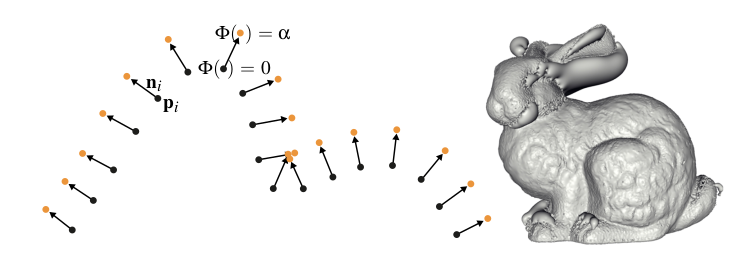
\includegraphics[scale=0.5]{images/4.png}
    \caption{(слева) Для RBFs оптимизируемое скалярное поле должно оцениваться как нуль в точках выборки $\Phi(\mathbf{p_i}) = 0$, в то время как при ограничениях вне поверхности $\Phi(\mathbf{p_i} + \alpha\mathbf{n_i}) = \alpha;$ этот выбор уместен, поскольку функции расстояния со знаком почти везде имеют норму единичного градиента. Кластер выборок вне поверхности показывает, насколько тщательно нужно задавать ограничения в областях с большой кривизной. (справа) Поверхность, реконструированная с помощью RBFs, обычно имеет серьезные геометрические и топологические артефакты, когда предоставляются противоречивые внешние ограничения.}
    \label{fig:4}
\end{figure}

\subsection{Метод движущихся наименьших квадратов}
Процедура определения поверхности методом наименьших квадратов была представлена Левином ~\cite{LEVIN}.
Пусть точки $p_i \in R^{3}, i \in \{1, . . . , N\}$, взяты с
поверхности S (возможно, с шумом измерения). Цель состоит в том, чтобы спроецировать точку $r \in R^{3}$ вблизи S на двумерную поверхность SP, аппроксимирующую $p_i$. Процедура MLS мотивирована дифференциальной геометрией, а именно тем, что поверхность может быть локально аппроксимирована функцией. Алгоритм называется движущимся, поскольку итеративно двигается по набору точек. Точка на которой находится итерация, называется точкой запроса. Для точки запроса r (см. рис. \ref{fig:0}) вычисляется локальная плоскость H с использованием метода наименьших квадратов по точкам попавшим в окрестность радиуса R (параметр алгоритма) 

Эталонная плоскость: 
 Локальная плоскость $ H = \{x \mid \langle n, x \rangle - D = 0, x  \in R^{3}\}, n \in R^{3},  \parallel n \parallel = 1 $ вычисляется так, чтобы минимизировать локальную взвешенную сумму квадратов расстояний точек $p_i$ до плоскости (см. рис. \ref{fig:0}). Веса, соответствующие $p_i$, определяются как функция расстояния от $p_i$ до проекции r на плоскость H, а не от расстояния до r. Предположим, что q является проекцией r на H, тогда H находится путем локальной минимизации
 \begin{equation}
     \sum_{i = 1}^{N}(\langle n, p_i \rangle - D)^{2} \theta(\parallel p_i - q \parallel)
     \label{eq:ref1}
 \end{equation}

где $\theta$ — гладкая монотонно убывающая функция, положительная на всем пространстве. Полагая $q = r + tn$ для некоторого $t \in R$, уравнение \ref{eq:ref1} можно переписать как: 
 $$\sum_{i = 1}^{N}(\langle n, p_i - r - tn \rangle)^{2} \theta(\parallel p_i - r - tn \parallel)$$
 
  Оператор $Q(r) = q = r + tn$ определяется как локальный минимум уравнения  с наименьшим t и локальной касательной плоскостью H вблизи r соответственно. Затем локальная эталонная область задается ортонормированной системой координат на H, так что q является началом этой системы. Затем вычисляется локальная полиномиальная аппроксимация g точек $p_i$ над H. Проекция точки запроса на полином является результатом работы алгоритма MLS.

\begin{figure}[h]
    \centering
    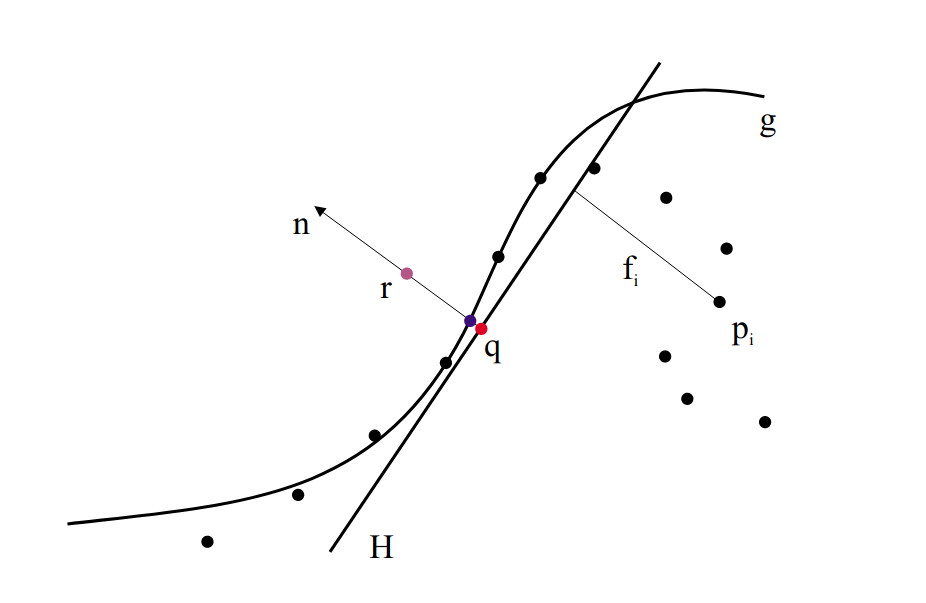
\includegraphics[scale=0.5]{images/0.png}
    \caption{Шаг алгоритма движущихся наименьших квадратов}
    \label{fig:0}
\end{figure}

\subsection{Повышение дискретизации и рендеринг}

Алгоритм MLS позволяет повысить плотность точек если плотность исходного облака точек недостаточна.  На плоскости $H$, найденной методом наименьших квадратов, задается набор точек на окружностях с заданным шагом и радиусом(см. рис. \ref{fig:upsampling}) которые в последствие проецируются на полином.

\begin{figure}[h]
  \centering
  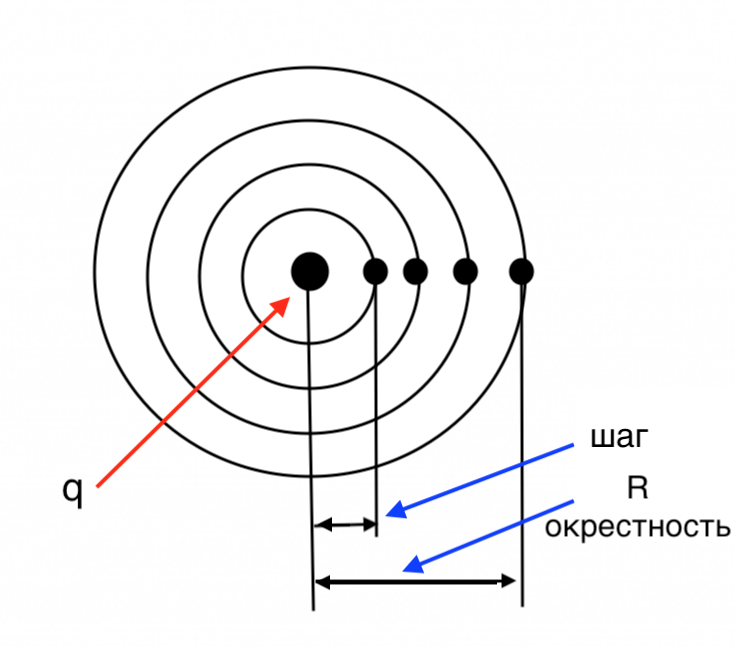
\includegraphics[width=0.42\textwidth, height=6cm]{images/rendering.png}
  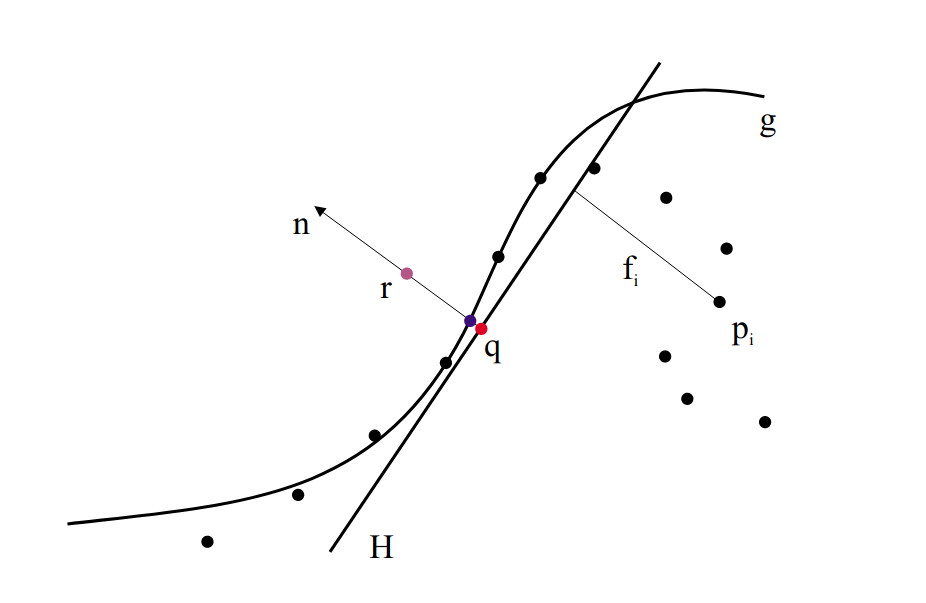
\includegraphics[width=0.56\textwidth, height=6cm]{images/0.png}
  \caption{Повышение плотности точек за счет проекции дополнительных точек выбранных на плоскости H.}
  \label{fig:upsampling}
\end{figure}

В 2000м году Шимон Русинкевич и Марк Левой предложили подход рендеринга при котором поверхность представляется набором точек и при необходимости повышается дискретизация до разрешения экрана ~\cite{Szymon}. Такой подход должен был обеспечить большую производительность ввиду отсутствия затрат на настройку и растеризацию полигонов. Но из-за значительного роста производительности графических устройств и того что рендеринг в таком программном обеспечение как Unity и Blender завязан на полигональных моделях, спустя 20 лет можно сказать что этот подход себя не оправдал.


\begin{figure}[h]
  \centering
  \subbottom[25000000 полигонов]{%
    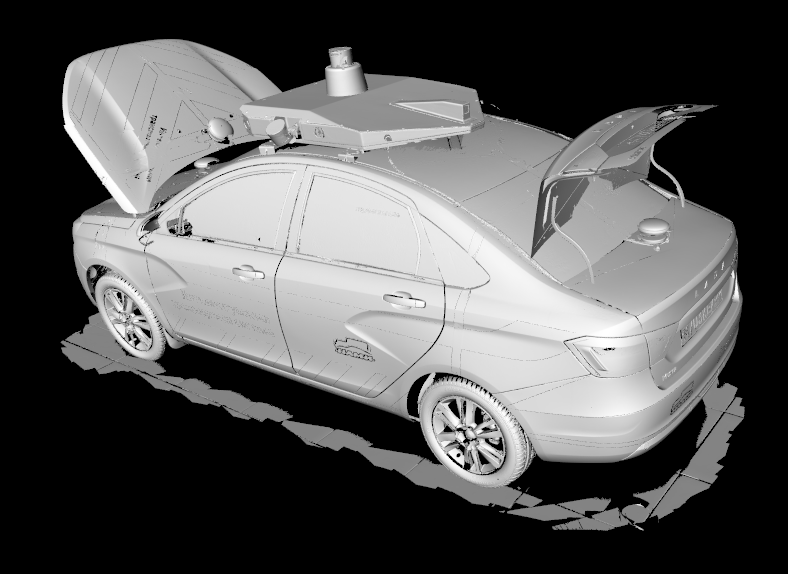
\includegraphics[width=0.49\textwidth, height=7cm]{images/polygon.png}}
  \subbottom[25000000 точек]{%
    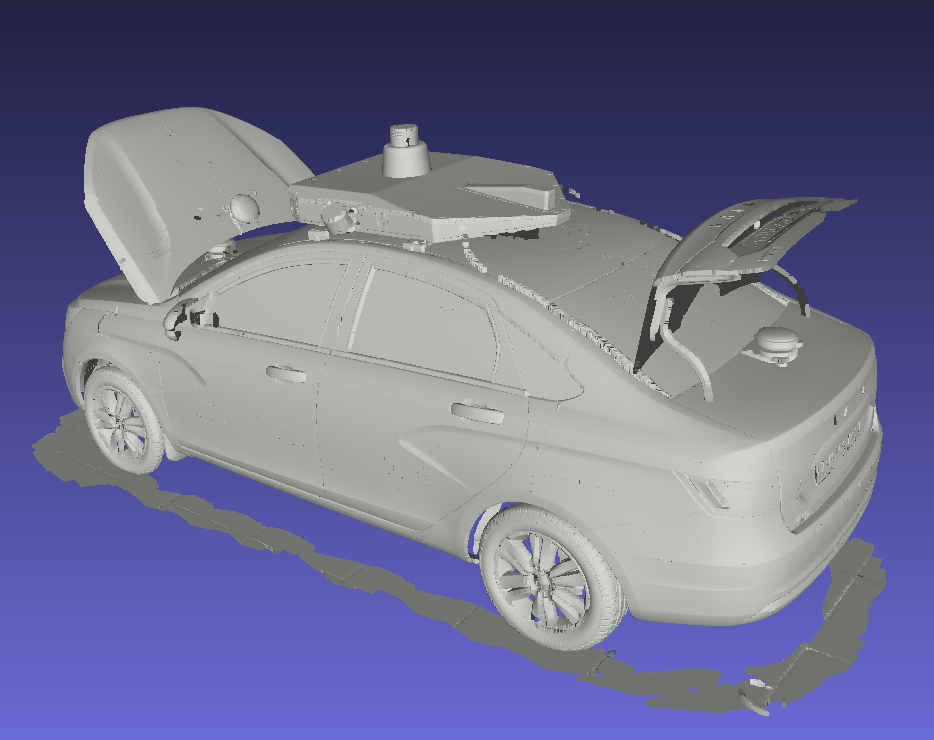
\includegraphics[width=0.49\textwidth, height=7cm]{images/point_set.png}}
  \caption{Сравнение рендеринга векторно-полигональной модели и поверхности представленной набором точек}
\end{figure}

    \section{Разработка параллельного алгоритма реконструкции поверхности}
\subsection{Предложенный параллельный метод}
Параллельный вариант, модифицированного алгоритма MLS с использованием MPI, описан в алгоритме 1. Алгоритм предполагает что облако точек равномерно распределено по всем процессам \ref{fig:decomposition}. Поэтому часть P, доступная локально в процессе u, обозначается через $P^{(u)}$. Через $P_l^{u}$, $P_r^{u}$ обозначены левая и правая граница частей облака точек. Они последовательно получаются от соседних процессов обменами по топологии кольцо. Дополнительных коммуникаций не требуется, а остальные вычисления выполняются локально. В цикле по локальному облаку точек $P^{(u)}$ выполняется процедура проецирования MLS: сначала создается локальная эталонная плоскость H для точки $p_j$. Проекция $p_j$ на H определяет начало координат q. Затем вычисляется локальная полиномиальная аппроксимация g высот $f_j$ точек $p_j$ над H. Проекция $p_j$ на g является результатом работы алгоритма MLS. \\*
\textbf{Алгоритм 1}  Параллельный метод движущихся наименьших квадратов с MPI и OpenMP \\*
\textbf{Вход:} набор точек $P = \{p_i\}$ $i = 1..n$ \\*
\textbf{Выход:} поверхность представленная набором точек \\*
1: \textbf{for each} process u \textbf{do} \\*
2: \quad $P^{(u)} = read(P)$ // каждый процесс считывает свой сегмент облака точек $P^{(u)} = \{p_j\}$ $j = 1..m$ \\*
3: \quad $P\_l^{(u)} = send\_recv(P\_r^{(u-1)})$ // получение левой границы\\* 
4: \quad $P\_r^{(u)} = send\_recv(P\_l^{(u+1)})$ // получение правой границы\\*
5: \quad\textbf{pragma omp parallel for} \\*
6: \quad\textbf{for each} point $j = 1..m $ \textbf{do}\\*
7: \quad\quad$H = generate\_plane(p_j)$ \\*
8: \quad\quad$g = generate\_local\_polynomial\_approximation(H)$ \\*
9: \quad\quad$result\_point = project\_on\_polynom(p_j, polynom)$ \\*
10: \quad\textbf{end for} \\*

При исследовании информационной структуры алгоритма был построен граф информационной зависимости \ref{fig:information}. Из графа видно отсутствие информационной зависимости между точками запроса, поэтому итерации по циклу из локального набора точек $P^{(u)}$ были распараллелены средствами OpenMP (строчка 5 алгоритма 1). 

\begin{figure}[h]
    \centering
    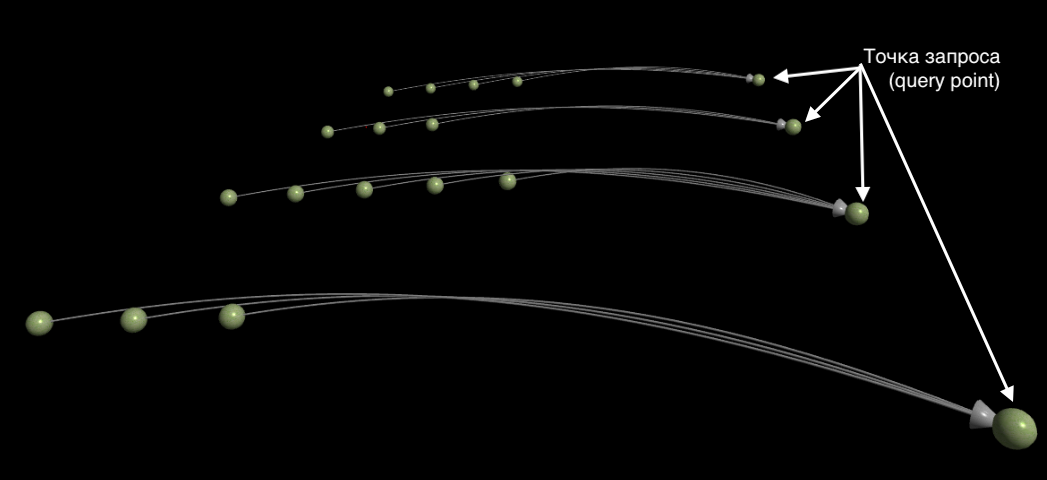
\includegraphics[width=0.7\textwidth, height=5cm]{images/graph.png}
    \caption{Граф информационной зависимости MLS.}
    \label{fig:information}
\end{figure}

\begin{figure}[h]
    \centering
    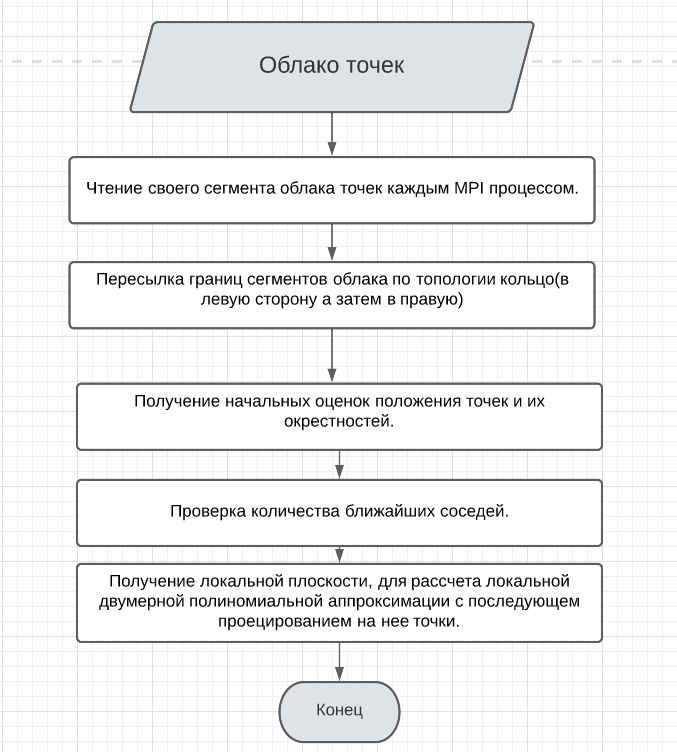
\includegraphics[scale=0.9]{1.png}
    \caption{Блок-схема параллельной реализации алгоритма}
    \label{fig:mesh1}
\end{figure}


\begin{figure}[h]
  \centering
  \subbottom[$np = 1$]{%
    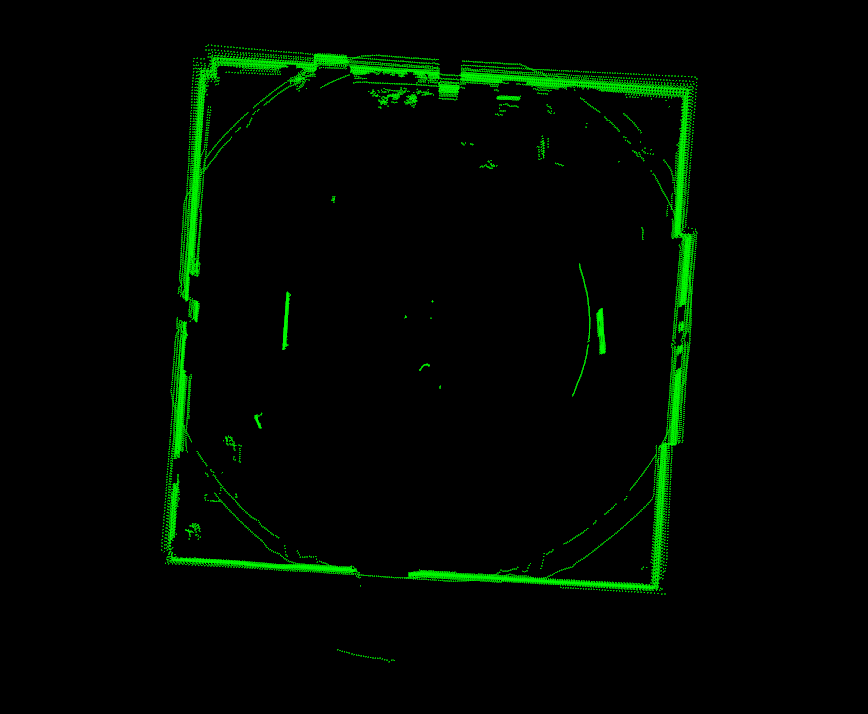
\includegraphics[width=0.4\textwidth, height=7cm]{images/3.png}}
  \subbottom[$np = 4$]{%
    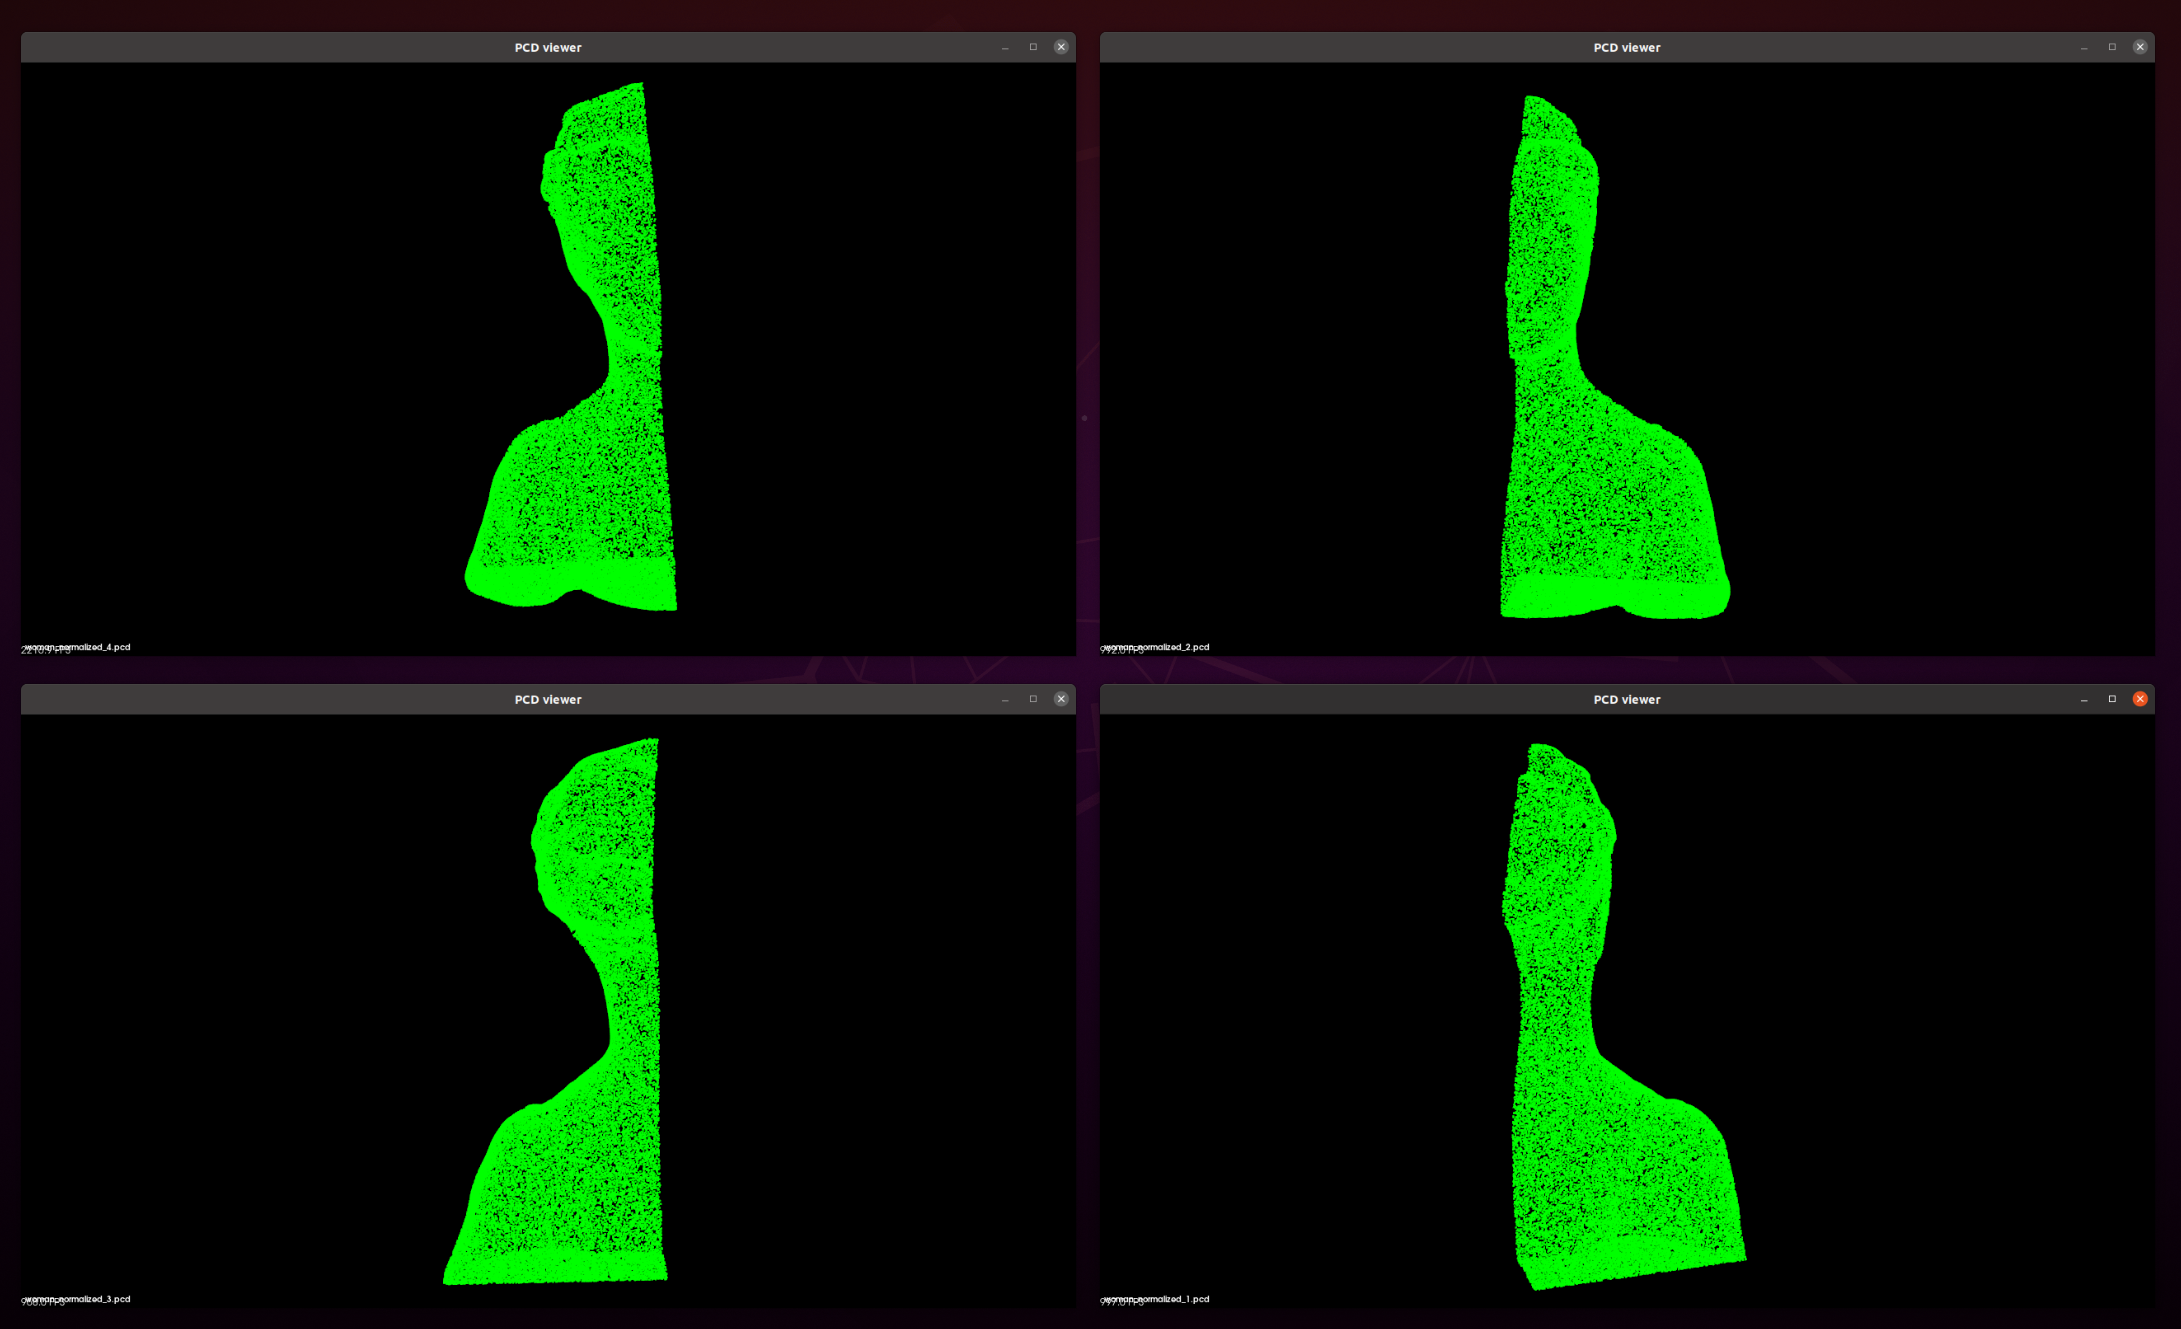
\includegraphics[width=0.58\textwidth, height=7cm]{images/2.png}}
  \caption{Распределение сегментов облака точек по процессам}
  \label{fig:decomposition}
\end{figure}

\clearpage



\subsection{Вычислительная сложность}
Для эффективного поиска точек попадающих в R окрестность используется структура данных k-d дерево. Вычислительная сложность построения k-d-дерева порядка: $O(n*k*log(n))$. Здесь k = 3 и имеет значение размерности. Несбалансированное k-d-дерево можно построить за $O(n(k+log(n)))$. У нас есть n точек, каждая вставляется за логарифмическую сложность. Слагаемое $O(nk)$ имеет следующее значение: Перед построением дерева находится минимум и максимум по каждой размерности для последующего равномерного разбиения. В случае сбалансированного дерева применяется предварительная сортировка по всем размерностям сложностью порядка $O(nlog n)$.
Поиск точек в окрестности R имеет сложность порядка $O(log n)$.
Метод наименьших квадратов для поиска плоскости имеет сложность порядка $O(C^2*m)$ $ (C = 4)$. Здесь С имеет значение количества параметров, и равно 4‑м поскольку мы ищем плоскость.
Интерполяция полиномом имеет сложность порядка $O(m^2)$, где m имеет значение количества точек попавших в R окрестность.

\begin{table}[h]
\centering
\begin{tabular}{||p{7cm}||p{9.3cm}||}
\hline
Этап алгоритма & сложность\\
\hline\hline
Построение k-d-дерева &  $O(n \cdot k \cdot log(n))$ (Несбалансированное $O(n(k+log(n)))$ ) \\
\hline
Поиск точек в окрестности R & $O(log n)$  \\
\hline
Метод наименьших квадратов & $O(C^2 \cdot m) (C = 4)$\\
\hline
Интерполяция полиномом & $O(m^2)$ \\
\hline
Проекция точки на полином & $O(1)$ \\
\hline
\end{tabular}
\caption{Вычислительная сложность основных этапов алгоритма}
\label{table:complexity}
\end{table}

Итоговая амортизационная вычислительная сложность алгоритма: 

$O(n \cdot k \cdot log(n))$  + n $\cdot$ ($O(log n)$ + $O(C^2 \cdot m)$ + $O(m^2)$ + $O(1)$)
    \section{Результаты вычислительных методов}

\subsection{Характеристики вычислительной системы для проведения экспериментов}

Спецификация системы: 

 Polus - параллельная вычислительная система, состоящая из 5 вычислительных узлов. (на первый вычислительный узел возложены функции frontend узла)
 
\noindent Основные характеристики каждого узла:
\begin{itemize}
    \item 2 десятиядерных процессора IBM POWER8 (каждое ядро имеет 8 потоков) всего 160 потоков
    \item Общая оперативная память 256 Гбайт (в узле 5 оперативная память 1024 Гбайт) с ЕСС контролем
    \item 2 х 1 ТБ 2.5” 7K RPM SATA HDD
    \item 2 x NVIDIA Tesla P100 GPU, 16Gb, NVLink
    \item 1 порт 100 ГБ/сек
\end{itemize}

\noindent Производительность кластера (Tflop/s): 55,84 (пиковая), 40,39 (Linpack) \\

\subsection{Описание экспериментов}
Рассмотрим теперь вопрос об эффективности алгоритма. Для этого напомним, что
каждый параллельный алгоритм оценивается по двум параметрам – ускорению $S_p$ и
эффективности $E_p$ , которые определяются по формулам:
$$S_p = {{t_1} \over {t_p}},$$ $$E_p = {S_p \over p} * 100\%$$
где $t_1$ - время решения исходной задачи на одном процессоре, $t_p$ - время
решения исходной задачи по параллельному алгоритму на p процессорах.

Для оценки работы алгоритма с точки зрения качества реконструкции поверхности были проведены следующие эксперименты:\\ 
Были взяты полигональные модели разные по сложности формы начиная от обычного куба и заканчивая морским ежом(см. рис. \ref{fig:polygonal models}). Все модели были предварительно нормированы следующим образом: сдвинуты центром масс к началу координат, все вершины модели были отмасштабированы так, что максимальное отклонение от начала координат было менее 1. Данные полигональные модели впоследствии будем называть эталонными.\\
С полигональных моделей были взяты 200000 случайных точек(см. рис. \ref{fig:point cloud models}).\\ 
Облако точек с эталонной модели зашумлялось аддитивным гауссовым шумом с различным среднеквадратичным отклонением. Данное облако точек впоследствии использовались в качестве входных данных алгоритма MLS.\\
К зашумленному облаку точек применялся алгоритм MLS с различным параметром $\bold{R}$. Восстановленная алгоритмом MLS поверхность представленная набором точек сравнивалась с эталонной моделью.
Были посчитаны среднее отклонение восстановленной поверхности от эталонной модели, а также среднеквадратичное отклонение (Таблицы \ref{table:1}, \ref{table:2}, \ref{table:3}, \ref{table:4}, \ref{table:5}, \ref{table:6}). По результатам исследований алгоритм MLS хорошо справляется с зашумленными данными, но для достижения оптимальных результатов нужно тщательно подбирать параметр радиуса алгоритма. Это особенно касается моделей сложной формы. Слишком маленький радиус может вести к потере данных ввиду невозможности найти локальную плоскость, а слишком большой ведет к размытию резких контуров поверхности.

\begin{figure}[h]
  \centering
    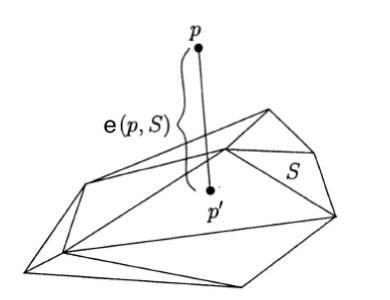
\includegraphics[width=0.8\textwidth]{images/distance.jpg}
  \caption{Отклонение $e_i(p, S)$ — это расстояние между точкой и поверхностью S. Точка $p^{'}$ — ближайшая точка к поверхности S.}
\end{figure}

\clearpage
\subsection{Картинки, таблицы, графики}

\begin{table}[h]
\begin{tabular}{|c|c|c|c|c|}
    \hline
    $R$ & Число MPI-процессов & Время работы (с) & Ускорение & Эффективность \\
    \hline
    0.0008 & 1 & 601.91  &  1  &  100.0 \\
    0.0008 & 2 & 356.632  &  1.69  &  84.39 \\
    0.0008 & 4 & 210.948  &  2.85  &  71.33 \\
    0.0008 & 8 & 124.986  &  4.82  &  60.2 \\
    0.0008 & 16 & 73.742  &  8.16  &  51.01 \\
    0.0008 & 32 & 43.434  &  13.86  &  43.31 \\
    \hline
    0.0012 &  1  &  1070.74  &  1  &  100.0 \\
    0.0012 &  2  &  615.675  &  1.74  &  86.96 \\
    0.0012 &  4  &  342.008  &  3.13  &  78.27 \\
    0.0012 &  8  &  193.405  &  5.54  &  69.2 \\
    0.0012 &  16  &  110.338  &  9.7  &  60.65 \\
    0.0012 &  32  &  63.003  &  17.0  &  53.11 \\
    \hline
    0.0016 &  1  &  1959.78  &  1  &  100.0 \\
    0.0016 &  2  &  1093.557  &  1.79  &  89.61 \\
    0.0016 &  4  &  579.585  &  3.38  &  84.53 \\
    0.0016 &  8  &  310.948  &  6.3  &  78.78 \\
    0.0016 &  16  &  168.845  &  11.61  &  72.54 \\
    0.0016 &  32  &  90.501  &  21.65  &  67.67 \\
    \hline
\end{tabular}
\caption{Результаты запуска программы для различных значений параметра R. На вход подавалось облако из 25000000 точек.}
\label{table:1}
\end{table}

На графиках представлены измерения для различных значений параметра R при изменении количества MPI процессов. Из графика эффективности видно, что при большем радиусе, эффективность падает медленнее. Это связано с увеличением количества локальных вычислений при тех же затратах на коммуникации между процессами.


\begin{figure}[h]
    \centering
    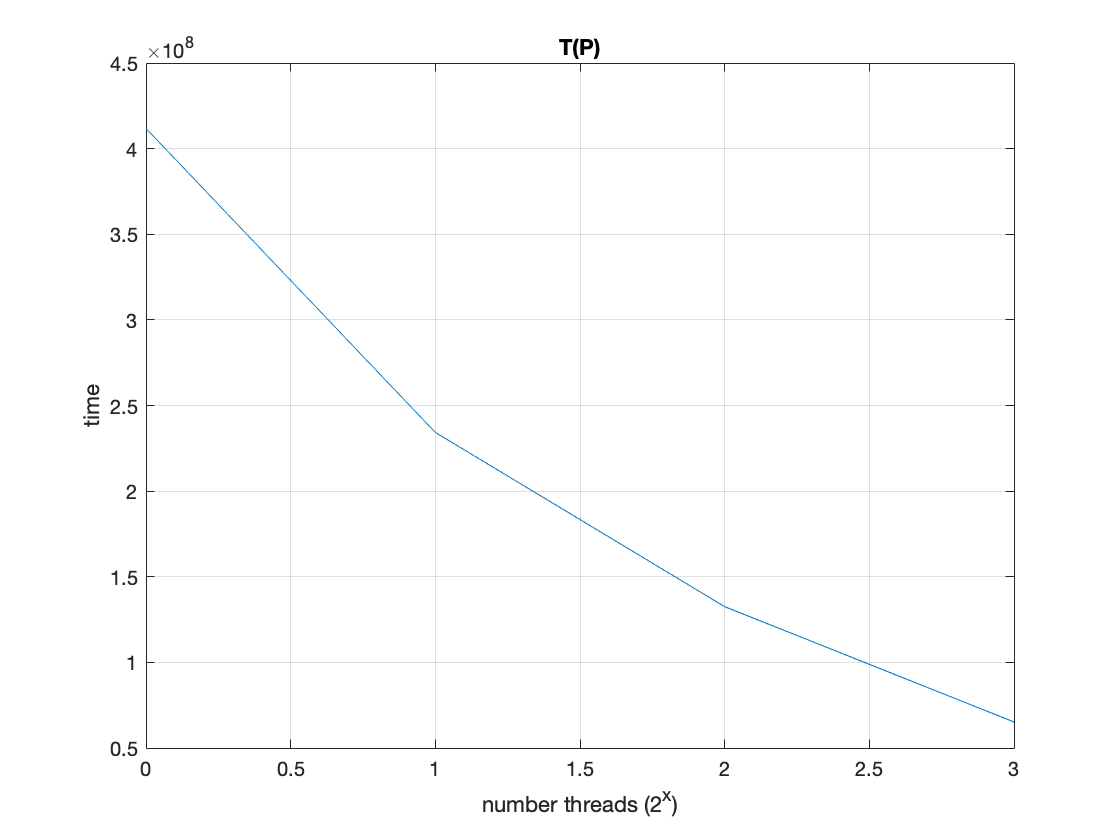
\includegraphics[scale=0.6]{T(P).png}
    \caption{Время работы (c) на n процессах n = 1...32}
    \label{fig:mesh1}
\end{figure}

\begin{figure}[h]
    \centering
    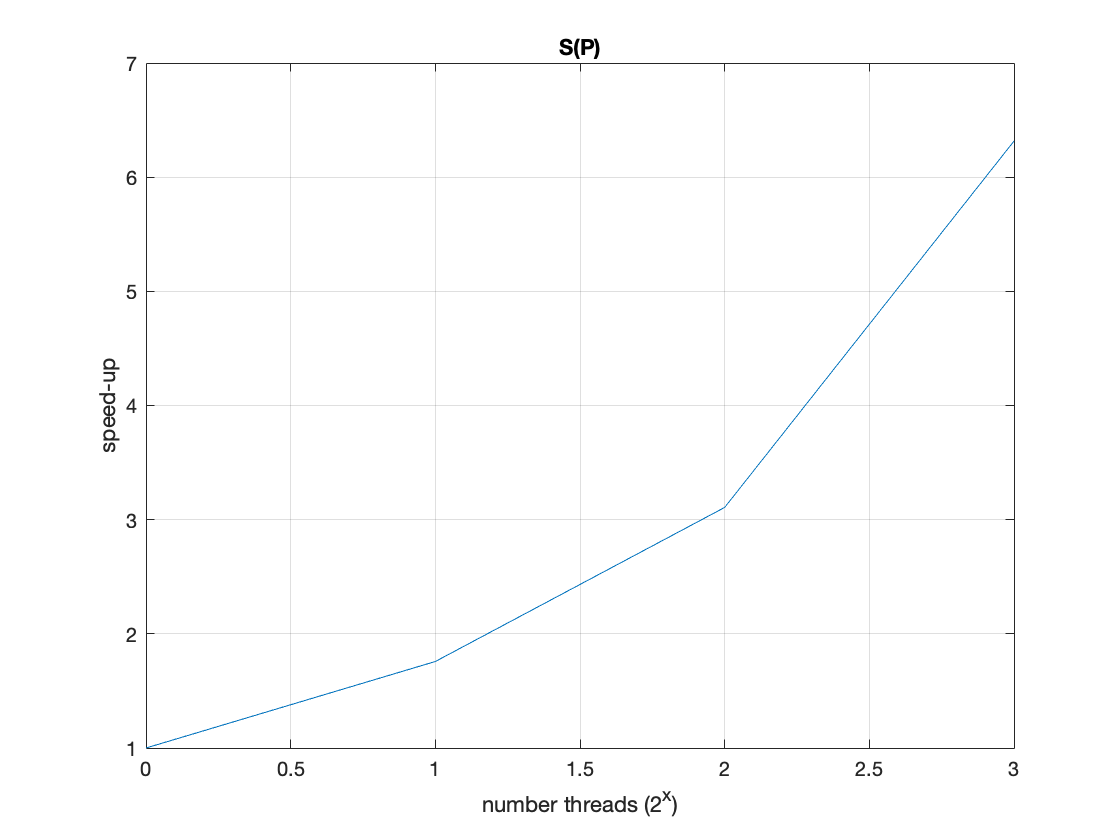
\includegraphics[scale=0.6]{S(P).png}
    \caption{Ускорение}
    \label{fig:mesh1}
\end{figure}

\begin{figure}[h]
    \centering
    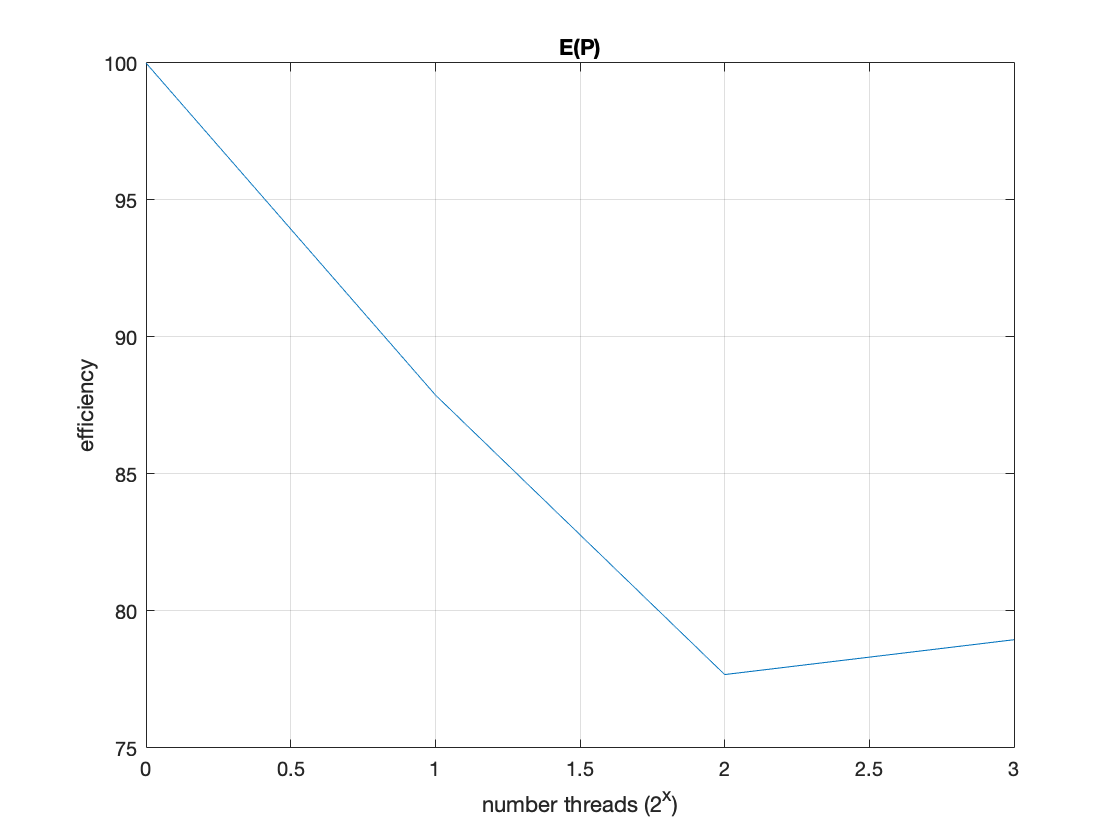
\includegraphics[scale=0.6]{E(P).png}
    \caption{Эффективность}
    \label{fig:mesh1}
\end{figure}

\begin{table}[h]
\begin{tabular}{|c|c|c|c|c|c|}
    \hline
    $R$ & Число MPI-процессов & Число OpenMP-нитей & Время работы (с)  \\
    \hline\hline
    0.0008 &  1  & 1  &  601.91 \\
    0.0008 &  2  & 1  &  356.632 \\
    0.0008 &  4  & 1  &  210.948 \\
    0.0008 &  8  & 1  &  124.986 \\
    \hline
    0.0008 &  1  & 2  &  340.348 \\
    0.0008 &  2  & 2  &  201.095 \\
    0.0008 &  4  & 2  &  117.203 \\
    0.0008 &  8  & 2  &  68.377 \\
    \hline
    0.0008 &  1  & 4  &  183.182 \\
    0.0008 &  2  & 4  &  108.107 \\
    0.0008 &  4  & 4  &  63.591 \\
    0.0008 &  8  & 4  &  37.494 \\
    \hline\hline
    0.0012 &  1  & 1  &  1070.74 \\
    0.0012 &  2  & 1  &  615.675 \\
    0.0012 &  4  & 1  &  342.008 \\
    0.0012 &  8  & 1  &  193.405 \\
    \hline
    0.0012 &  1  & 2  &  602.795 \\
    0.0012 &  2  & 2  &  340.879 \\
    0.0012 &  4  & 2  &  187.004 \\
    0.0012 &  8  & 2  &  104.702 \\
    \hline
    0.0012 &  1  & 4  &  310.09 \\
    0.0012 &  2  & 4  &  176.728 \\
    0.0012 &  4  & 4  &  97.626 \\
    0.0012 &  8  & 4  &  55.051 \\
    \hline\hline
    0.0016 &  1  & 1  &  1959.78 \\
    0.0016 &  2  & 1  &  1093.557 \\
    0.0016 &  4  & 1  &  579.585 \\
    0.0016 &  8  & 1  &  310.948 \\
    \hline
    0.0016 &  1  & 2  &  1080.297 \\
    0.0016 &  2  & 2  &  598.387 \\
    0.0016 &  4  & 2  &  312.359 \\
    0.0016 &  8  & 2  &  166.638 \\
    \hline
    0.0016 &  1  & 4  &  558.458 \\
    0.0016 &  2  & 4  &  310.34 \\
    0.0016 &  4  & 4  &  163.279 \\
    0.0016 &  8  & 4  &  87.274 \\
    
    \hline
\end{tabular}
\caption{Результаты запуска гибридной программы для различных значений параметра R. На вход подавалось облако из 25000000 точек.}
\label{table:1}
\end{table}

\clearpage
На следующем графике представлены измерения времени работы для различных значений параметра R при изменении количества mpi процессов c применением openMP. По итогу гибридная программа оказалась эффективней чисто MPI программы.

\begin{figure}[h]
    \centering
    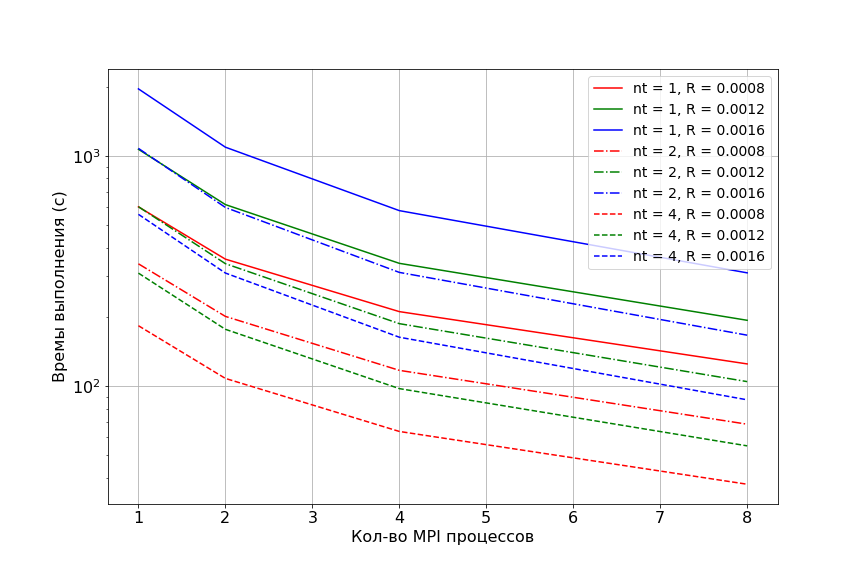
\includegraphics[scale=0.6]{images/time_1_omp.png}
    \caption{Время работы гибридной программы (MPI + OpenMP)}
    \label{fig:mesh1}
\end{figure}

\clearpage
Все полигональные модели были нормированы для того чтобы результаты на разных моделях были сравнимыми. Полигональная модель состоит из перечисления вершин и связей между ними. Для нормирования полигональной модели достаточно нормировать облако точек вершин. Связи между вершинами при этом остаются без изменений.

\begin{figure}[h]
    \centering
    \subbottom[Cube]{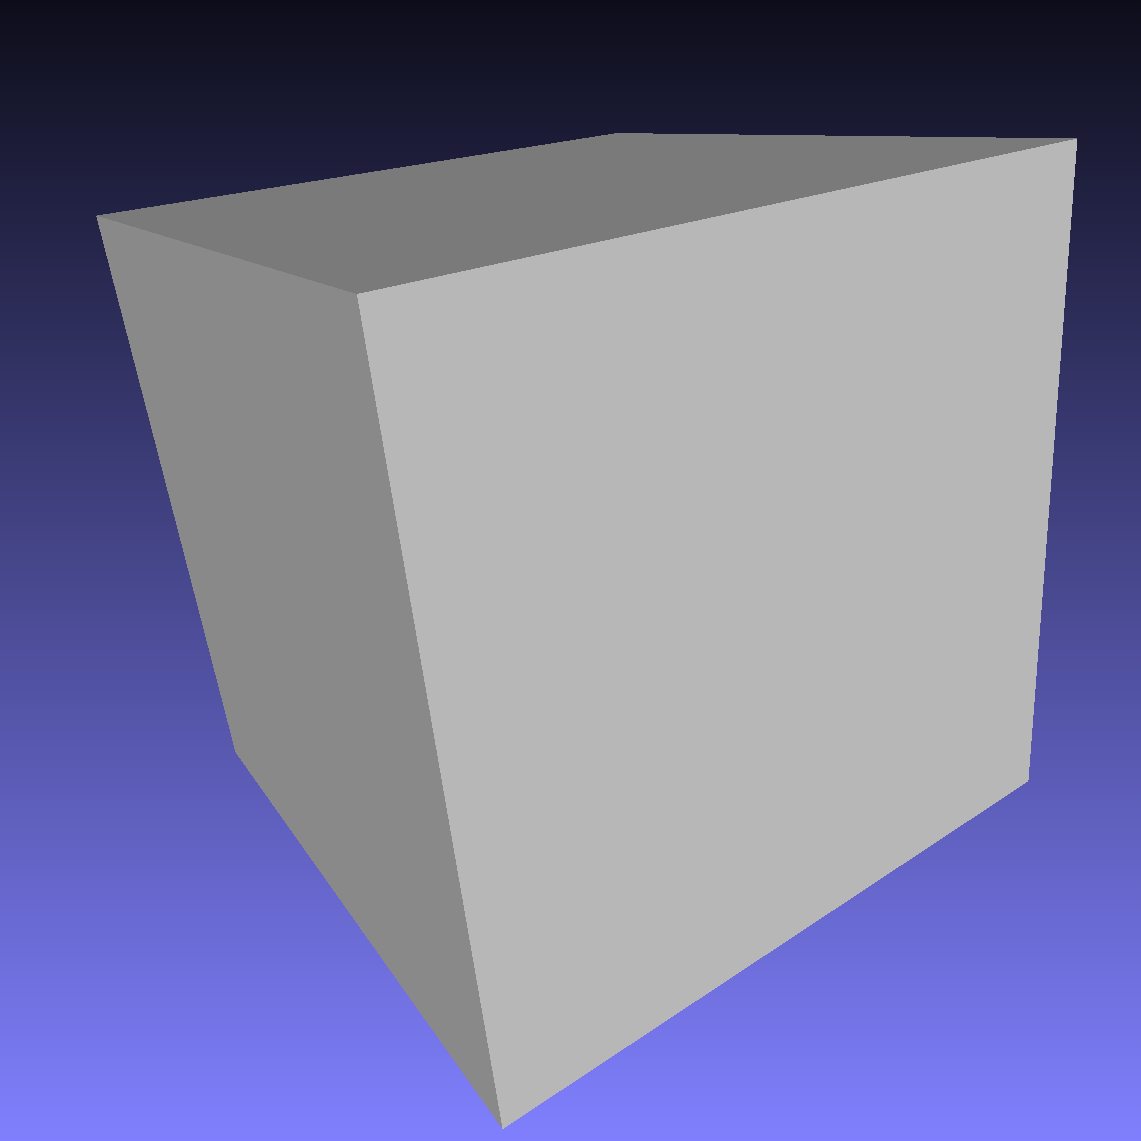
\includegraphics[width=0.32\textwidth, height=5cm]{ply/cube.png}}
    \subbottom[Woman]{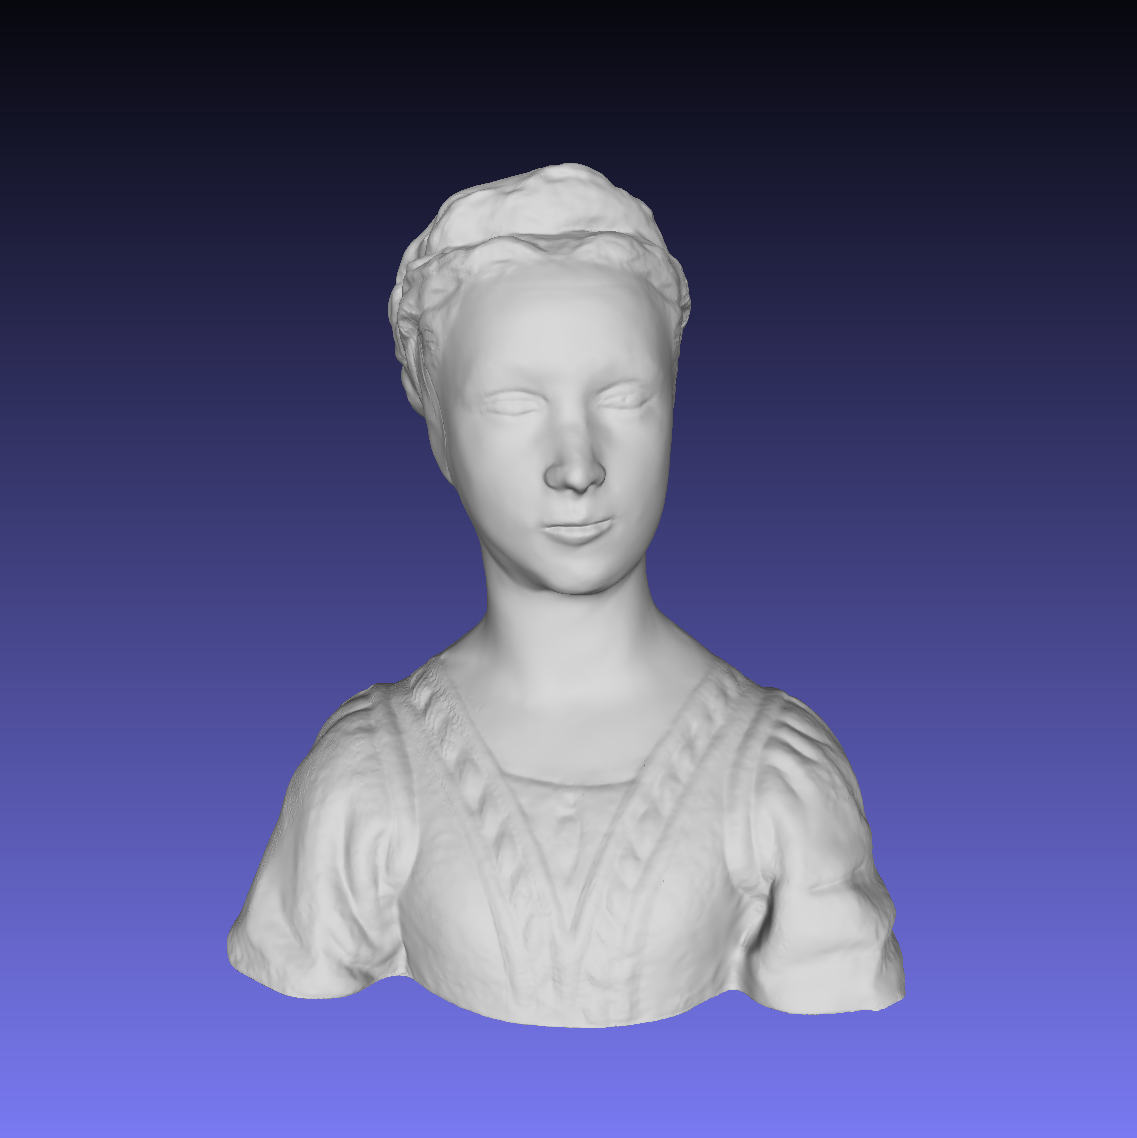
\includegraphics[width=0.32\textwidth, height=5cm]{ply/woman.png}}
    \subbottom[Elephant]{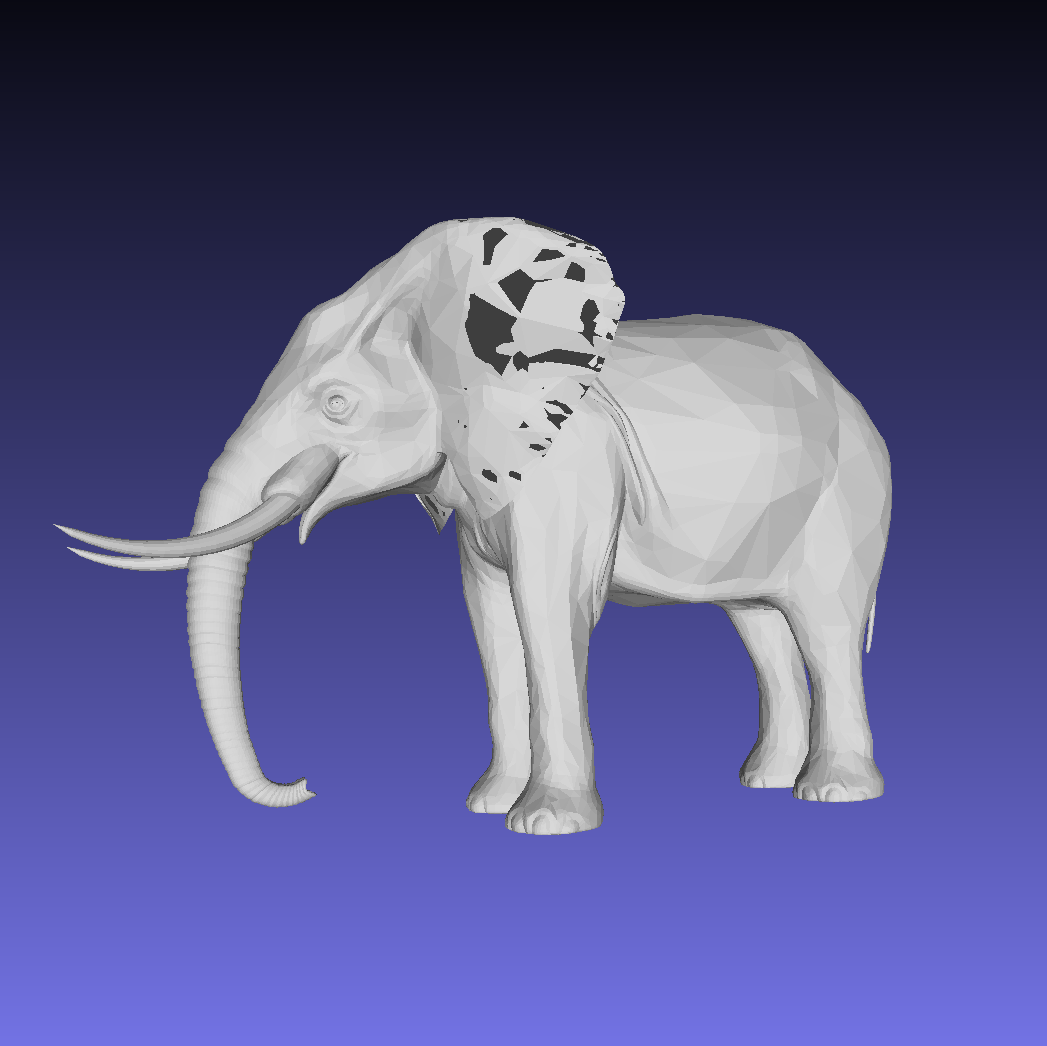
\includegraphics[width=0.32\textwidth, height=5cm]{ply/elephant.png}}
    \subbottom[Hippo]{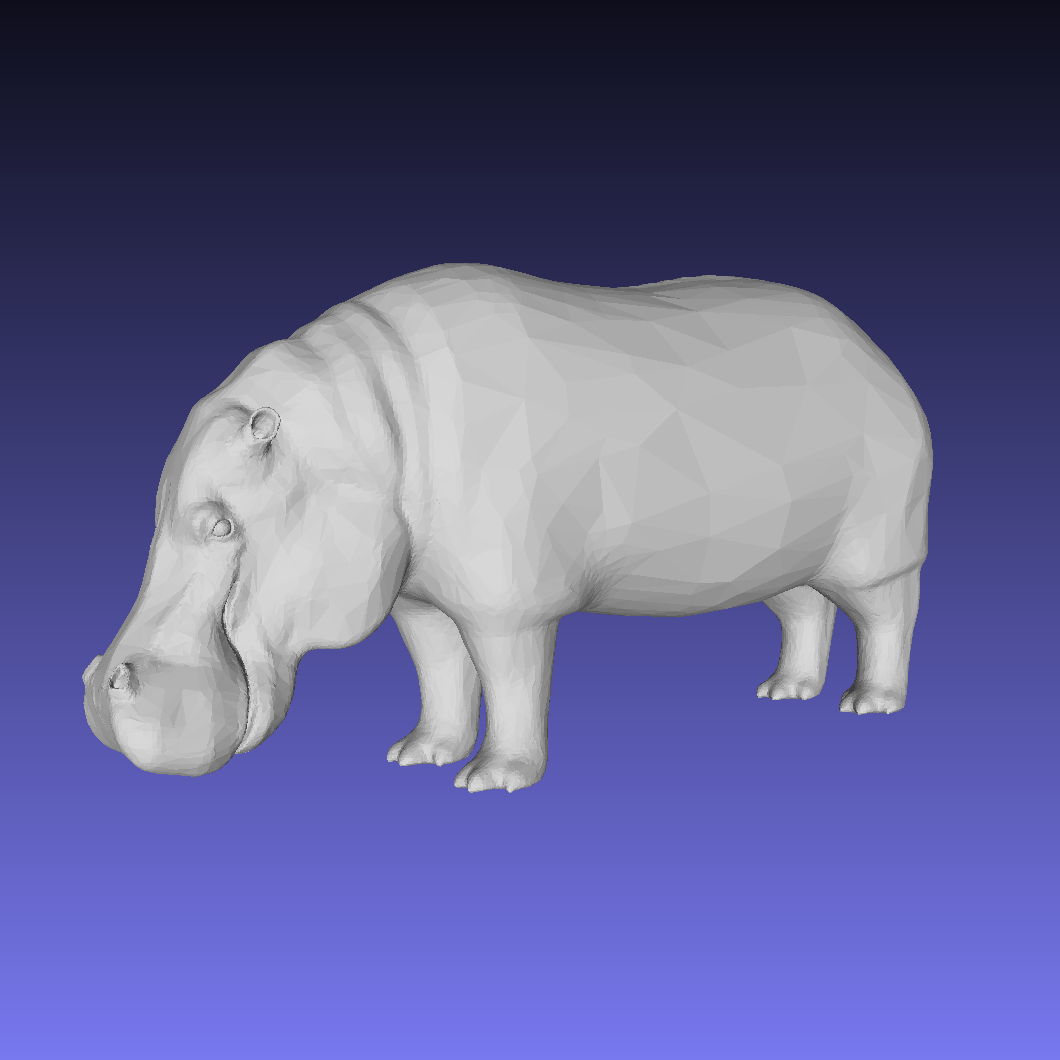
\includegraphics[width=0.32\textwidth, height=5cm]{ply/hippo.png}}
    \subbottom[Bunny]{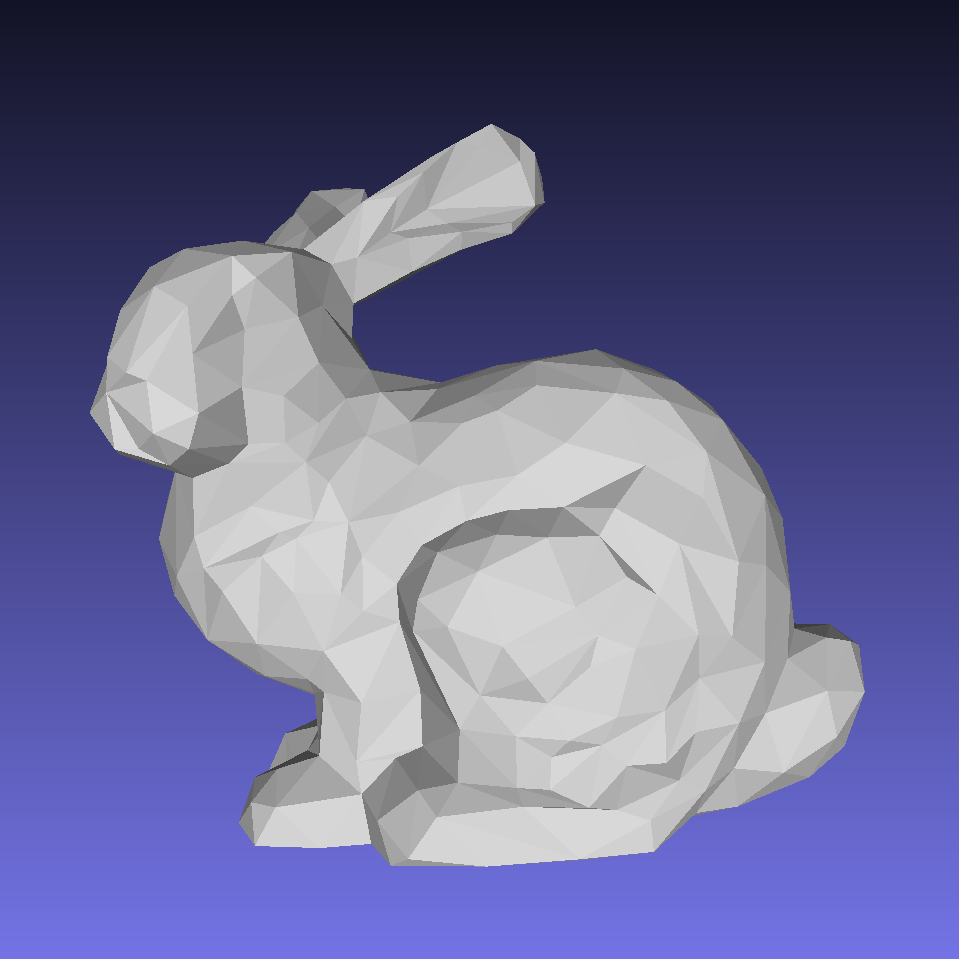
\includegraphics[width=0.32\textwidth, height=5cm]{ply/bunny.png}}
    \subbottom[Sea Urchin]{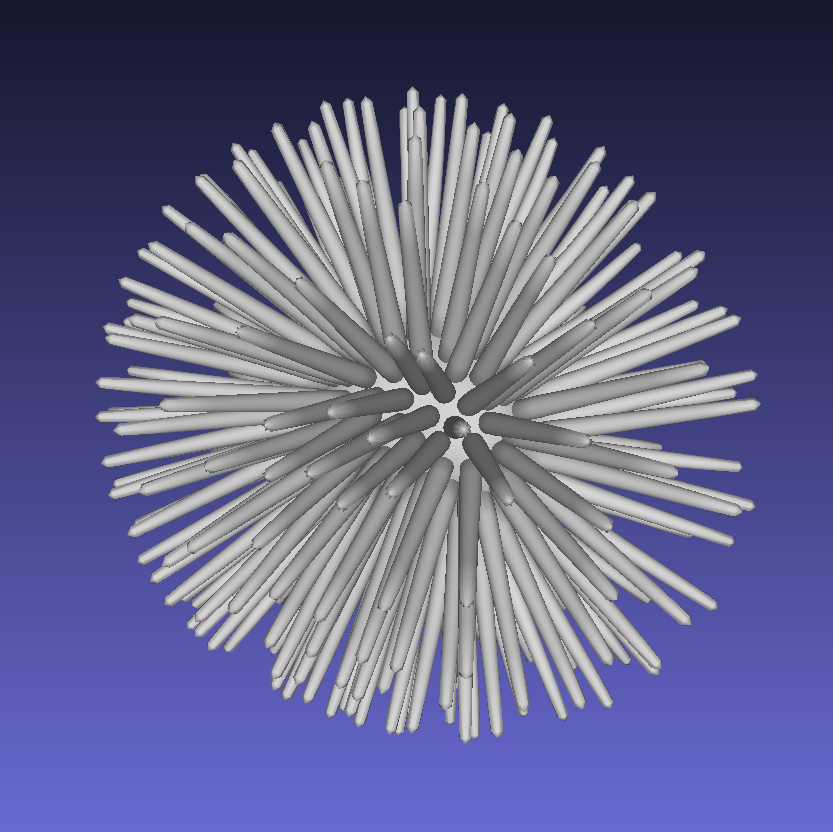
\includegraphics[width=0.32\textwidth, height=5cm]{ply/sea_urchin.png}}
    \caption{Полигональные модели для тестирования качества работы алгоритма.}
    \label{fig:polygonal models}
\end{figure}

\begin{figure}[h]
    \centering
    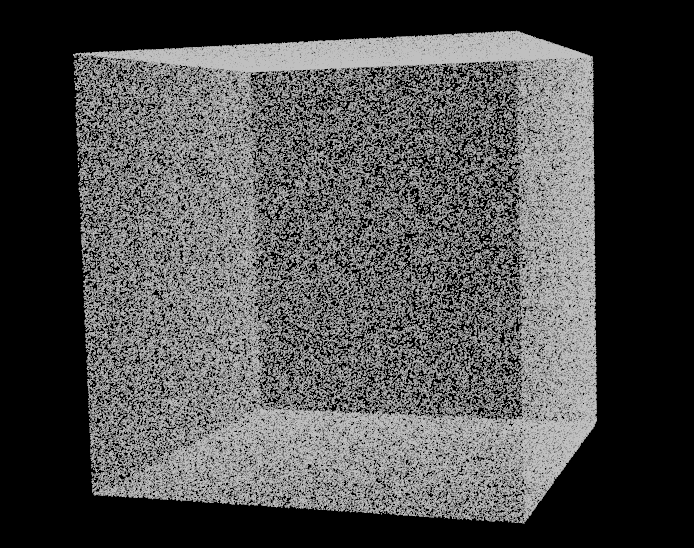
\includegraphics[width=0.32\textwidth, height=5cm]{pcd/cube.png}
    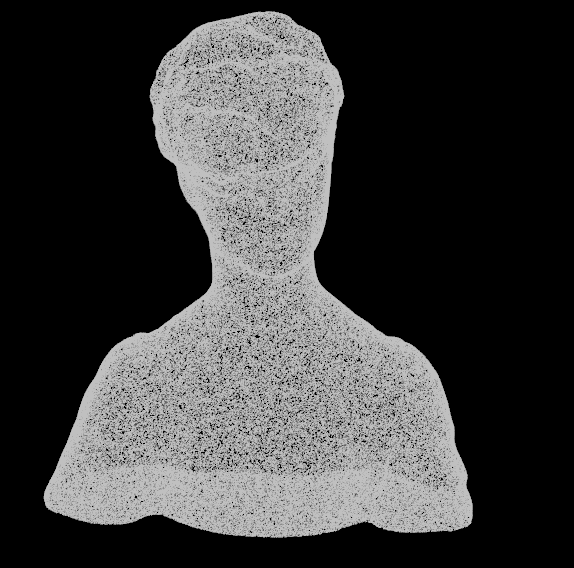
\includegraphics[width=0.32\textwidth, height=5cm]{pcd/woman.png}
    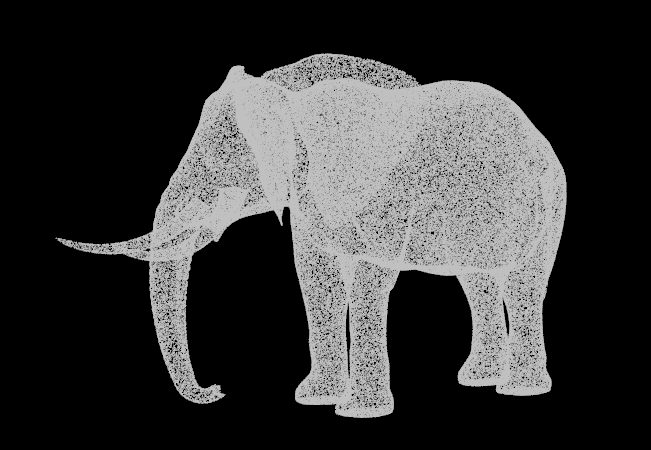
\includegraphics[width=0.32\textwidth, height=5cm]{pcd/elephant.png}
    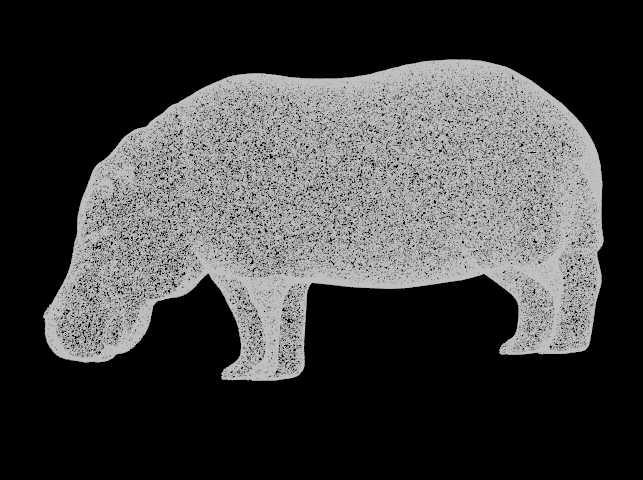
\includegraphics[width=0.32\textwidth, height=5cm]{pcd/hippo.png}
    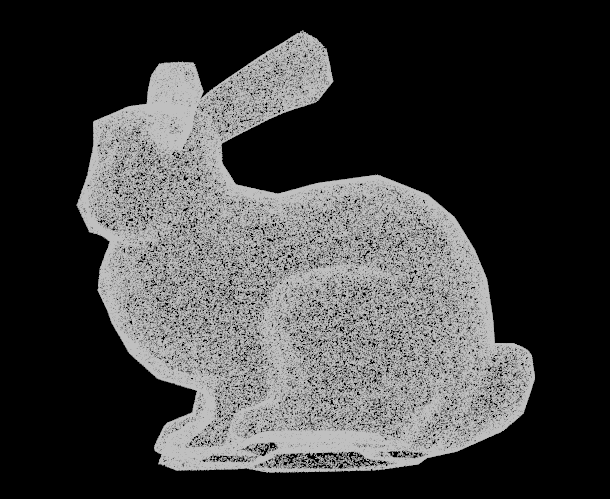
\includegraphics[width=0.32\textwidth, height=5cm]{pcd/bunny.png}
    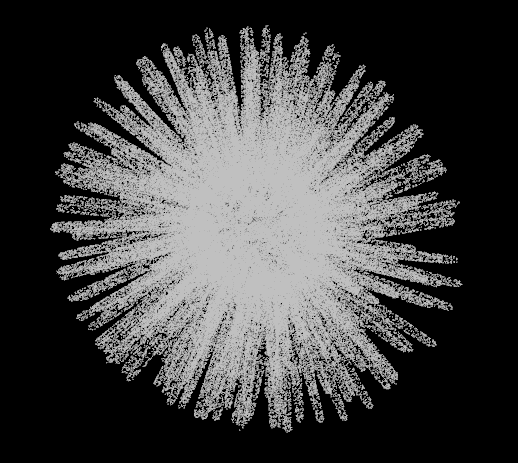
\includegraphics[width=0.32\textwidth, height=5cm]{pcd/sea_urchin.png}
    \caption{Облака точек взятые с полигональных моделей. С каждой модели взято 200000 рандомных точек.}
    \label{fig:point cloud models}
\end{figure}

\begin{figure}[h]
  \centering
  \subbottom[зашумленное облако точек с модели Bunny]{%
    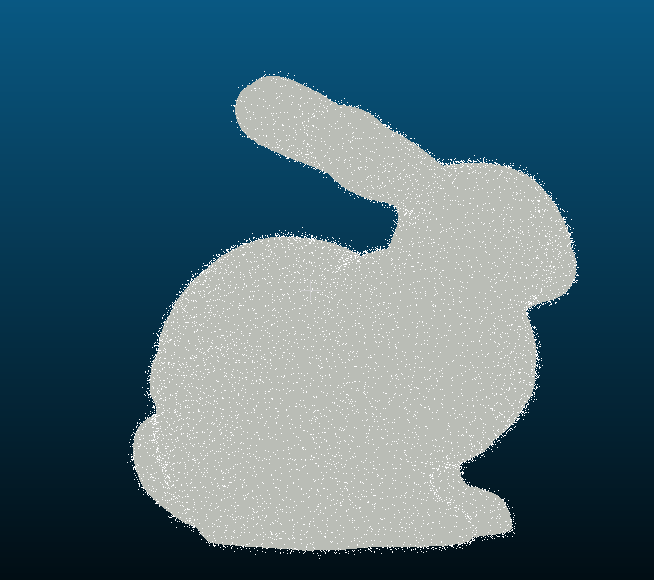
\includegraphics[width=8cm]{images/bunnyWithNoise.png}}
  \subbottom[Bunny после MLS]{%
    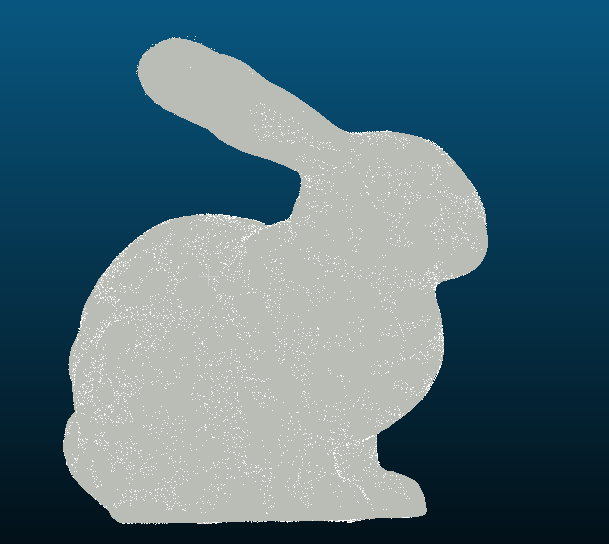
\includegraphics[width=8cm]{images/bynnyAfterMLS.png}}
  \caption{Слева зашумленное облако точек аддитивным Гауссовым шумом с $\boldsymbol{\sigma = 0.01}$ на эталонной поверхности. Справа, восстановленное облако точек методом MLS на той же эталонной поверхности.}
\end{figure}

\begin{figure}[h]
  \centering
  \subbottom[зашумленное облако точек с модели Bunny]{%
    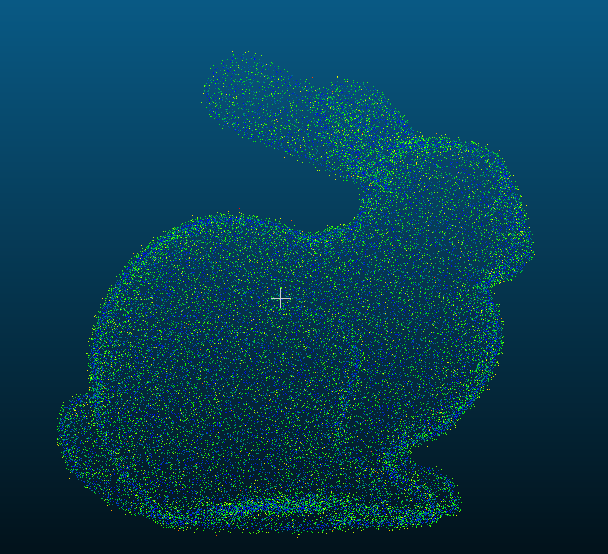
\includegraphics[width=0.49\textwidth, height=8cm]{images/bunnyWithNoiseCompare.png}}
  \subbottom[Bunny после MLS]{%
    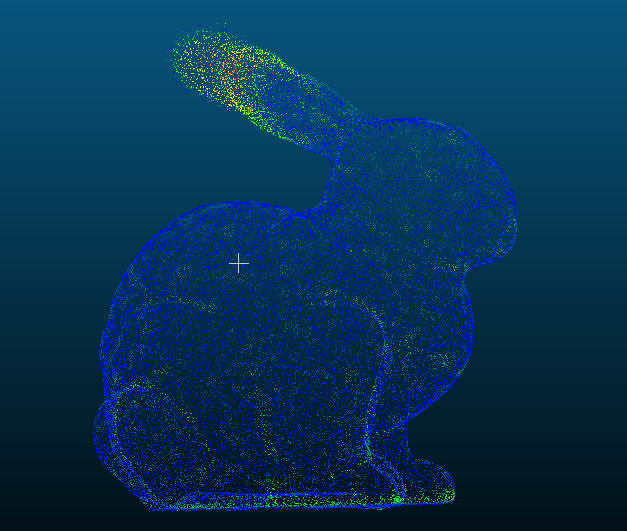
\includegraphics[width=0.49\textwidth, height=8cm]{images/bunnyAfterMLSCompare.png}}
  \caption{Слева зашумленное облако точек аддитивным Гауссовым шумом с $\boldsymbol{\sigma = 0.01}$. Справа, восстановленное облако точек методом MLS. Интенсивность цвета обозначает величину отклонения от эталонной поверхности.}
\end{figure}

В таблицах \ref{table:1}, \ref{table:2}, \ref{table:3}, \ref{table:4}, \ref{table:5}, \ref{table:6} представлены измерения для различных моделей. Цель измерений была установить положительное влияние алгоритма движущихся наименьших квадратов и  подобрать оптимальный свободный параметр (Радиус окрестности). Для всех моделей за исключением Sea Urchin (рис. \ref{fig:polygonal models} (f)) видно, что значение радиуса нужно подбирать немного больше значения среднеквадратичного отклонения шума. Это хорошая начальная оценка учитывая большой набор методов оценки распределения шума. Более точное значение параметра можно подобрать исходя из визуальной оценки используя к примеру кнопку ползунок.  Также стоит отметить для большинства моделей наличие локального минимума до значения среднеквадратичного отклонения шума. Это связано с тем, что алгоритм MLS, выбрасывает из результата те точки, для которых нашлось менее 3‑х соседей, считая такие точки выбросами. При подборе достаточно маленького радиуса это ведет к значительной потере данных.
\begin{table}[h]
\centering
\begin{tabular}{| c | c | c| c | c | c | c |}
    \hline
    применен MLS & $\sigma$ & $\bold{R}$ & ср. геом. откл. & ср. кв. откл. & min & max \\
    \hline\hline
    $\times$ & 0.005 & -- & 0.00484 & 0.00269 & 3.8e-05 & 0.0245\\
    \checkmark & 0.005 &  0.005 & 0.00372 & 0.00181 & 5.5e-05 & 0.01418\\
    \checkmark & 0.005 &  0.01 & 0.00434 & 0.00245 & 6.7e-05 & 0.01715\\
    \checkmark & 0.005 &  0.03 & \textbf{0.00248} & \textbf{0.00117} & 3.5e-05 & 0.01676\\
    \checkmark & 0.005 &  0.05 & 0.00277 & 0.00185 & 1.3e-05 & 0.02362\\
    \hline
    $\times$ & 0.01 & -- & 0.00854 & 0.00563 & 0.0001 & 0.04387\\
    \checkmark & 0.01 &  0.005 & 0.00578 & 0.00339 & 6.2e-05 & 0.02481\\
    \checkmark & 0.01 &  0.01 & 0.00741 & 0.0045 & 8.7e-05 & 0.03055\\
    \checkmark & 0.01 &  0.03 & \textbf{0.00334} & \textbf{0.002} & 9e-06 & 0.04387\\
    \checkmark & 0.01 &  0.05 & 0.00344 & 0.00226 & 6.1e-05 & 0.03942\\
    \hline
    $\times$ & 0.03 & -- & 0.02333 & 0.01722 & 0.000167 & 0.13393\\
    \checkmark & 0.03 &  0.005 & 0.01424 & 0.01001 & 0.000167 & 0.06133\\
    \checkmark & 0.03 &  0.01 & 0.01672 & 0.01168 & 0.000158 & 0.07857\\
    \checkmark & 0.03 &  0.03 & 0.02065 & 0.01572 & 0.00012 & 0.10811\\
    \checkmark & 0.03 &  0.05 & \textbf{0.01284} & \textbf{0.01116} & 8.3e-05 & 0.11659\\
    \hline
\end{tabular}

\caption{Результат работы алгоритма MLS на модели Bunny. На вход алгоритма подается облако точек с модели, зашумленное аддитивным гауссовым шумом. Сравнивается восстановленная поверхность MLS c различным параметром R с эталонной поверхностью по среднему отклонению (mean distance), среднеквадратичному отклонению (standard deviation), минимальному (min) и максимальному (max) отклонению.  $\bold{R}$ -- параметр алгоритма MLS, $\sigma$ -- среднеквадратичное отклонение аддитивного гауссового шума.}
\label{table:1}
\end{table}


\begin{table}[h]
\centering
\begin{tabular}{| c | c | c| c | c | c | c |}
    \hline
    применен MLS & $\sigma$ & $\bold{R}$ & ср. геом. откл. & ср. кв. откл. & min & max \\
    \hline\hline
    $\times$ & 0.005 & -- & 0.00528 & 0.00266 & 9e-05 & 0.0231\\
    \checkmark & 0.005 &  0.005 & 0.00394 & 0.00176 & 0.000173 & 0.01341\\
    \checkmark & 0.005 &  0.01 & 0.00481 & 0.00229 & 6.1e-05 & 0.01872\\
    \checkmark & 0.005 &  0.03 & \textbf{0.00312} & \textbf{0.00143} & 5.6e-05 & 0.01069\\
    \checkmark & 0.005 &  0.05 & 0.00323 & 0.00149 & 2.1e-05 & 0.01071\\
    \hline
    $\times$ & 0.01 & -- & 0.00896 & 0.00553 & 6.3e-05 & 0.04574\\
    \checkmark & 0.01 &  0.005 & 0.00608 & 0.00321 & 0.000239 & 0.02309\\
    \checkmark & 0.01 &  0.01 & 0.00722 & 0.00395 & 7e-05 & 0.03011\\
    \checkmark & 0.01 &  0.03 & 0.00423 & 0.00242 & 7.1e-05 & 0.04506\\
    \checkmark & 0.01 &  0.05 & \textbf{0.00363} & \textbf{0.00172} & 3e-05 & 0.01496\\
    \hline
    $\times$ & 0.03 & -- & 0.02413 & 0.0175 & 5.5e-05 & 0.13091\\
    \checkmark & 0.03 &  0.005 & 0.01506 & 0.01012 & 0.000453 & 0.06424\\
    \checkmark & 0.03 &  0.01 & 0.01603 & 0.01086 & 0.00022 & 0.08114\\
    \checkmark & 0.03 &  0.03 & 0.02172 & 0.01601 & 7.2e-05 & 0.10536\\
    \checkmark & 0.03 &  0.05 & \textbf{0.0139} & \textbf{0.0122} & 0.000107 & 0.1205\\
    \hline
\end{tabular}

\caption{Результат работы алгоритма MLS на модели Cube. На вход алгоритма подается облако точек с модели, зашумленное аддитивным гауссовым шумом. Сравнивается восстановленная поверхность MLS c различным параметром R с эталонной поверхностью по среднему отклонению (mean distance), среднеквадратичному отклонению (standard deviation), минимальному (min) и максимальному (max) отклонению.  $\bold{R}$ -- параметр алгоритма MLS, $\sigma$ -- среднеквадратичное отклонение аддитивного гауссового шума.}
\label{table:2}
\end{table}


\begin{table}[h]
\centering
\begin{tabular}{| c | c | c| c | c | c | c |}
    \hline
    применен MLS & $\sigma$ & $\bold{R}$ & ср. геом. откл. & ср. кв. откл. & min & max \\
    \hline\hline
    $\times$ & 0.005 & -- & 0.00477 & 0.00268 & 6.1e-05 & 0.02512\\
    \checkmark & 0.005 &  0.005 & 0.00368 & 0.00181 & 6.1e-05 & 0.01509\\
    \checkmark & 0.005 &  0.01 & 0.00424 & 0.00244 & 5.8e-05 & 0.0187\\
    \checkmark & 0.005 &  0.03 & \textbf{0.00265} & \textbf{0.00151} & 4.6e-05 & 0.01855\\
    \checkmark & 0.005 &  0.05 & 0.00301 & 0.00236 & 2.2e-05 & 0.02479\\
    \hline
    $\times$ & 0.01 & -- & 0.00836 & 0.00559 & 0.000109 & 0.04483\\
    \checkmark & 0.01 &  0.005 & 0.00574 & 0.00343 & 0.00012 & 0.02845\\
    \checkmark & 0.01 &  0.01 & 0.00731 & 0.0045 & 5.5e-05 & 0.03267\\
    \checkmark & 0.01 &  0.03 & \textbf{0.00347} & \textbf{0.00222} & 3.8e-05 & 0.04305\\
    \checkmark & 0.01 &  0.05 & 0.00372 & 0.00268 & 6e-05 & 0.03384\\
    \hline
    $\times$ & 0.03 & -- & 0.02264 & 0.01693 & 9.1e-05 & 0.1461\\
    \checkmark & 0.03 &  0.005 & 0.01384 & 0.01005 & 0.000269 & 0.07674\\
    \checkmark & 0.03 &  0.01 & 0.01659 & 0.01172 & 0.000124 & 0.08642\\
    \checkmark & 0.03 &  0.03 & 0.02005 & 0.01549 & 8.6e-05 & 0.10592\\
    \checkmark & 0.03 &  0.05 & \textbf{0.01301} & \textbf{0.01142} & 4.4e-05 & 0.12447\\
    \hline
\end{tabular}

\caption{Результат работы алгоритма MLS на модели Elephant. На вход алгоритма подается облако точек с модели, зашумленное аддитивным гауссовым шумом. Сравнивается восстановленная поверхность MLS c различным параметром R с эталонной поверхностью по среднему отклонению (mean distance), среднеквадратичному отклонению (standard deviation), минимальному (min) и максимальному (max) отклонению.  $\bold{R}$ -- параметр алгоритма MLS, $\sigma$ -- среднеквадратичное отклонение аддитивного гауссового шума.}
\label{table:3}
\end{table}


\begin{table}[h]
\centering
\begin{tabular}{| c | c | c| c | c | c | c |}
    \hline
    применен MLS & $\sigma$ & $\bold{R}$ & ср. геом. откл. & ср. кв. откл. & min & max \\
    \hline\hline
    $\times$ & 0.005 & -- & 0.00477 & 0.00271 & 7.4e-05 & 0.02114\\
    \checkmark & 0.005 &  0.005 & 0.00366 & 0.00181 & 5.3e-05 & 0.01381\\
    \checkmark & 0.005 &  0.01 & 0.00422 & 0.00247 & 5e-05 & 0.01848\\
    \checkmark & 0.005 &  0.03 & \textbf{0.00234} & \textbf{0.00112} & 4e-05 & 0.01742\\
    \checkmark & 0.005 &  0.05 & 0.00243 & 0.00146 & 3.6e-05 & 0.01932\\
    \hline
    $\times$ & 0.01 & -- & 0.00846 & 0.00564 & 0.000118 & 0.04645\\
    \checkmark & 0.01 &  0.005 & 0.00579 & 0.00346 & 0.000106 & 0.02456\\
    \checkmark & 0.01 &  0.01 & 0.00742 & 0.00458 & 0.000103 & 0.03196\\
    \checkmark & 0.01 &  0.03 & \textbf{0.00287} & \textbf{0.00177} & 5e-05 & 0.0449\\
    \checkmark & 0.01 &  0.05 & 0.00299 & 0.00182 & 3.9e-05 & 0.02826\\
    \hline
    $\times$ & 0.03 & -- & 0.02364 & 0.01744 & 0.000117 & 0.1768\\
    \checkmark & 0.03 &  0.005 & 0.01462 & 0.01046 & 0.000183 & 0.07097\\
    \checkmark & 0.03 &  0.01 & 0.01719 & 0.01197 & 8.8e-05 & 0.0872\\
    \checkmark & 0.03 &  0.03 & 0.0208 & 0.01593 & 3.7e-05 & 0.1069\\
    \checkmark & 0.03 &  0.05 & \textbf{0.01255} & \textbf{0.01104} & 0.0001 & 0.12441\\
    \hline
\end{tabular}

\caption{Результат работы алгоритма MLS на модели Hippo. На вход алгоритма подается облако точек с модели, зашумленное аддитивным гауссовым шумом. Сравнивается восстановленная поверхность MLS c различным параметром R с эталонной поверхностью по среднему отклонению (mean distance), среднеквадратичному отклонению (standard deviation), минимальному (min) и максимальному (max) отклонению.  $\bold{R}$ -- параметр алгоритма MLS, $\sigma$ -- среднеквадратичное отклонение аддитивного гауссового шума.}
\label{table:4}
\end{table}


\begin{table}[h]
\centering
\begin{tabular}{| c | c | c| c | c | c | c |}
    \hline
    применен MLS & $\sigma$ & $\bold{R}$ & ср. геом. откл. & ср. кв. откл. & min & max \\
    \hline\hline
    $\times$ & 0.005 & -- & 0.00624 & 0.00275 & 7.3e-05 & 0.02333\\
    \checkmark & 0.005 &  0.005 & \textbf{0.00445} & \textbf{0.00185} & 9.3e-05 & 0.0123\\
    \checkmark & 0.005 &  0.01 & 0.00526 & 0.0022 & 6.9e-05 & 0.01588\\
    \checkmark & 0.005 &  0.03 & 0.00562 & 0.00254 & 9e-05 & 0.02307\\
    \checkmark & 0.005 &  0.05 & 0.00894 & 0.00436 & 0.00017 & 0.02779\\
    \hline
    $\times$ & 0.01 & -- & 0.00956 & 0.00486 & 0.000123 & 0.04262\\
    \checkmark & 0.01 &  0.005 & \textbf{0.00683} & \textbf{0.00305} & 0.000456 & 0.01841\\
    \checkmark & 0.01 &  0.01 & 0.00752 & 0.00341 & 0.000226 & 0.02633\\
    \checkmark & 0.01 &  0.03 & 0.00863 & 0.0045 & 5.9e-05 & 0.03821\\
    \checkmark & 0.01 &  0.05 & 0.01034 & 0.00485 & 7e-05 & 0.04272\\
    \hline
    $\times$ & 0.03 & -- & 0.01812 & 0.01358 & 0.000175 & 0.1198\\
    \checkmark & 0.03 &  0.005 & \textbf{0.01033} & \textbf{0.00584} & 0.000688 & 0.05006\\
    \checkmark & 0.03 &  0.01 & 0.01103 & 0.00631 & 0.000276 & 0.05743\\
    \checkmark & 0.03 &  0.03 & 0.01652 & 0.01145 & 0.000153 & 0.09185\\
    \checkmark & 0.03 &  0.05 & 0.01624 & 0.01225 & 0.000219 & 0.09817\\
    \hline
\end{tabular}

\caption{Результат работы алгоритма MLS на модели Sea Urchin. На вход алгоритма подается облако точек с модели, зашумленное аддитивным гауссовым шумом. Сравнивается восстановленная поверхность MLS c различным параметром R с эталонной поверхностью по среднему отклонению (mean distance), среднеквадратичному отклонению (standard deviation), минимальному (min) и максимальному (max) отклонению.  $\bold{R}$ -- параметр алгоритма MLS, $\sigma$ -- среднеквадратичное отклонение аддитивного гауссового шума.}
\label{table:5}
\end{table}


\begin{table}[h]
\centering
\begin{tabular}{| c | c | c| c | c | c | c |}
    \hline
    применен MLS & $\sigma$ & $\bold{R}$ & ср. геом. откл. & ср. кв. откл. & min & max \\
    \hline\hline
    $\times$ & 0.005 & -- & 0.00486 & 0.00269 & 6.7e-05 & 0.0226\\
    \checkmark & 0.005 &  0.005 & 0.00371 & 0.00179 & 7.6e-05 & 0.01491\\
    \checkmark & 0.005 &  0.01 & 0.00437 & 0.00245 & 8.7e-05 & 0.01768\\
    \checkmark & 0.005 &  0.03 & \textbf{0.00248} & \textbf{0.00113} & 3.8e-05 & 0.01193\\
    \checkmark & 0.005 &  0.05 & 0.00256 & 0.00125 & 3.1e-05 & 0.01736\\
    \hline
    $\times$ & 0.01 & -- & 0.00856 & 0.00564 & 8.3e-05 & 0.0453\\
    \checkmark & 0.01 &  0.005 & 0.0058 & 0.00336 & 0.000122 & 0.0258\\
    \checkmark & 0.01 &  0.01 & 0.00741 & 0.00447 & 3.8e-05 & 0.03209\\
    \checkmark & 0.01 &  0.03 & 0.00329 & 0.00186 & 3e-05 & 0.04396\\
    \checkmark & 0.01 &  0.05 & \textbf{0.00313} & \textbf{0.0016} & 3.4e-05 & 0.02138\\
    \hline
    $\times$ & 0.03 & -- & 0.02359 & 0.01737 & 7.6e-05 & 0.14377\\
    \checkmark & 0.03 &  0.005 & 0.01461 & 0.01033 & 0.000214 & 0.06379\\
    \checkmark & 0.03 &  0.01 & 0.01675 & 0.01164 & 6.5e-05 & 0.09195\\
    \checkmark & 0.03 &  0.03 & 0.0208 & 0.01587 & 0.000106 & 0.10975\\
    \checkmark & 0.03 &  0.05 & \textbf{0.0124} & \textbf{0.01011} & 3.2e-05 & 0.12571\\
    \hline
\end{tabular}

\caption{Результат работы алгоритма MLS на модели Woman. На вход алгоритма подается облако точек с модели, зашумленное аддитивным гауссовым шумом. Сравнивается восстановленная поверхность MLS c различным параметром R с эталонной поверхностью по среднему отклонению (mean distance), среднеквадратичному отклонению (standard deviation), минимальному (min) и максимальному (max) отклонению.  $\bold{R}$ -- параметр алгоритма MLS, $\sigma$ -- среднеквадратичное отклонение аддитивного гауссового шума.}
\label{table:6}
\end{table}


    %!TEX root = ../surface_reconstruction.tex

\section{Результаты работы}

В работе сформулирован и реализован параллельный алгоритм рекострукции поверхности с использованием программного интерфейса Message Passing Interface для передачи сообщений, завязанный на алгоритме движущихся наименьших квадратов. Алгоритм предусматривает равномерное распределение сегментов облака точек по процессам с последующей пересылкой границ разбиения по топологии кольцо. Все последующие вычисления выполняются локально. Будучи избавленным от последующих пересылок данных, он обеспечивает максимальное ускорение. 
}


% Информация о годе выполнения работы
\def\Year{%
    % 2006%
    \the\year%     % Текущий год
}

% Укажите тип работы
% Например:
%     Выпускная квалификационная работа,
%     Магистерская диссертация,
%     Курсовая работа, реферат и т.п.
\def\WorkType{%
    % Выпускная квалификационная работа%
    % Магистерская диссертация%
    % Курсовая работа%
    % Реферат%
    Магистерская диссертация%
}

% Название работы
%%%%%%%%%%% ВНИМАНИЕ! %%%%%%%%%%%%%%%%
% В МГУ ОНО ДОЛЖНО В ТОЧНОСТИ
% СООТВЕТСТВОВАТЬ ВЫПИСКЕ ИЗ ПРИКАЗА
% УТОЧНИТЕ НАЗВАНИЕ В УЧЕБНОЙ ЧАСТИ
\def\Title{%
    Исследование эффективности метода движущихся наименьших квадратов при реконструкции трёхмерной поверхности на суперкомпьютере%
}


% Имя автора работы
\def\Author{%
    Хабибулин Марат Ильдарович%
}

% Информация о научном руководителе
%% Фамилия Имя Отчество%
\def\SciAdvisor{%
    Никольский Илья Михайлович%
}
%% В формате: И.~О.~Фамилия%
\def\SciAdvisorShort{%
    И.~М.~Никольский%
}
%% должность научного руководителя
\def\Position{%
    % профессор%
    доцент%
    % старший преподаватель%
    % преподаватель%
    % ассистент%
    % ведущий научный сотрудник%
    % старший научный сотрудник%
    % научный сотрудник%
    % младший научный сотрудник%
}
%% учёная степень научного руководителя
\def\AcademicDegree{%
    % д.ф.-м.н.%
    % д.т.н.%
    к.ф.-м.н.%
    % к.т.н.%
    % без степени%
}

% Информация об организации, в которой выполнена работа
%% Город
\def\Place{%
    Москва%
}
%% Университет
\def\Univer{%
    Московский государственный университет имени М.~В.~Ломоносова%
}
%% Факультет
\def\Faculty{%
    Факультет вычислительной математики и кибернетики%
}
%% Кафедра    
\def\Department{%
    Кафедра суперкомпьютеров и квантовой информатики%
}     

%%%% Переключите статус документа для отладки
%%%% В режиме draft документ собирается очень быстро
%%%% и выводится полезная информация о том
%%%% какие строки вылезают за границы документа, что удобно для борьбы с ними
\def\Status{%
    % draft%
    final%
}

%%%% Включает и выключает подпись <<С текстом работы ознакомлен>>
\def\EnableSign{%
     true%
}
